\documentclass[11pt]{article}
\usepackage[T1]{fontenc}
\usepackage{lmodern}
\usepackage[margin=1in]{geometry}
\usepackage{amsmath,amssymb,amsthm,mathtools}
\usepackage{microtype,enumitem}
\usepackage{xcolor}
\usepackage{tikz}
\usetikzlibrary{arrows.meta,positioning,fit,backgrounds,calc}
\usepackage[colorlinks=true,linkcolor=blue!45!black,citecolor=green!35!black,urlcolor=blue!55!black]{hyperref}
\hypersetup{pdftitle={Perfect completeness for 2-to-1 games},pdfauthor={OpenAI},
  pdfsubject={Perfect-completeness hardness for exact 2-to-1 projection games},
  bookmarksdepth=2}
\ifdefined\pdfinfoomitdate\pdfinfoomitdate=1\fi
\ifdefined\pdftrailerid\pdftrailerid{}\fi
\ifdefined\pdfsuppressptexinfo\pdfsuppressptexinfo=15\fi
\newcommand{\F}{\mathbb F_2}
\newcommand{\E}{\mathbb E}
\newcommand{\Prob}{\mathbb P}
\newcommand{\one}{\mathbf 1}
\newcommand{\eps}{\varepsilon}
\DeclareMathOperator{\TV}{TV}
\DeclareMathOperator{\val}{val}
\DeclareMathOperator{\Span}{span}
\DeclareMathOperator{\rank}{rank}
\DeclareMathOperator{\im}{im}
\DeclareMathOperator{\Hom}{Hom}
\DeclareMathOperator{\supp}{supp}
\DeclareMathOperator{\Ann}{Ann}
\DeclareMathOperator{\Mat}{Mat}
\newtheorem{theorem}{Theorem}[section]
\newtheorem{lemma}[theorem]{Lemma}
\newtheorem{proposition}[theorem]{Proposition}
\newtheorem{corollary}[theorem]{Corollary}
\theoremstyle{definition}
\newtheorem{definition}[theorem]{Definition}
\newtheorem{example}[theorem]{Example}
\theoremstyle{remark}
\newtheorem{remark}[theorem]{Remark}
\numberwithin{equation}{section}
\allowdisplaybreaks[1]
\setlength{\emergencystretch}{2em}
\title{Perfect completeness for 2-to-1 games}
\author{OpenAI}
\date{September 23, 2026}
\begin{document}
\maketitle
\begin{abstract}
We prove the 2-to-1 Games Conjecture with perfect completeness.
For every fixed rational $\delta\in(0,1)$, it is NP-hard to distinguish
satisfiable 2-to-1 games from games of value at most $\delta$, with a fixed
alphabet and an explicitly listed unweighted multiset of constraints.
\end{abstract}
\section{Introduction}\label{sec:introduction}

A \emph{projection game} consists of a finite bipartite multigraph with disjoint
vertex sets $U,V$, a nonempty multiset $E$ of edge occurrences, finite answer
sets at its vertices, and a map $\pi_e$ from the left answer set to the right
answer set for each occurrence $e=(u,v)$.
A labeling chooses one answer at each vertex and satisfies $e$ when the right
answer equals the image of the left answer under $\pi_e$.
The \emph{value} of the game is the maximum fraction of satisfied occurrences.
Parallel occurrences may have different projection maps.

A \emph{2-to-1 game} has a common left alphabet $[2q]$ and right alphabet $[q]$,
where $[m]=\{1,\ldots,m\}$, and
\[
             |\pi_e^{-1}(b)|=2
        \qquad(e\in E,\ b\in[q]).
\]
Khot introduced the games conjectures in the study of hardness of
approximation~\cite{Khot2002}.  His original formulation allowed fibers
of size at most two; we use the exact-two convention.  The 2-to-1 Games
Conjecture asks for
NP-hardness of distinguishing satisfiable games from games of arbitrarily
small fixed value.  The satisfiable case is the \emph{perfect-completeness}
requirement: one labeling must satisfy every constraint.  Completeness
$1-\eps$ for each fixed $\eps>0$ does not itself give this endpoint, since
those reductions need not produce any finite satisfiable game.
There is also an obstruction to amplifying a constant gap by ordinary
repetition: repeating an exact-two projection $k$ times gives $2^k$
preimages of every right answer.  We prove the conjecture while retaining
two-element fibers, in the following explicit form.

\begin{theorem}\label{thm:main}
For every fixed rational $\delta\in(0,1)$ there are an integer $q=q(\delta)\ge2$
and a deterministic polynomial-time reduction from $3$-SAT to 2-to-1 games
with alphabets $[2q]$ and $[q]$ such that:
\begin{enumerate}[label=\textup{(\roman*)}]
\item a satisfiable formula produces a game of value $1$;
\item an unsatisfiable formula produces a game of value at most $\delta$.
\end{enumerate}
The output contains a nonempty explicit list of unweighted edge occurrences
and an explicit table for every projection map.
Every table has exactly two preimages for each right answer.
The polynomial running-time bound is in the ordinary binary input length;
its degree and constants may depend on the fixed $\delta$.
\end{theorem}

The theorem supplies the hypothesis of several perfect-completeness
reductions.  We derive consequences for maximum $k$-colorable subgraph
and satisfiable Not-Two constraints below, identifying those already
known unconditionally.

\subsection{Historical context and ingredients}

Austrin, O'Donnell, Tan and Wright established perfect-completeness 2-to-1
Label Cover hardness with alphabets of sizes $6$ and $3$ and soundness
$23/24+\eps$~\cite[Theorem~1.3, author manuscript]{AustrinODonnellTanWright2014}.
The remaining issue was to make soundness arbitrarily small while retaining
both perfect completeness and two-element fibers.

The near-perfect-completeness theorem arose from the Grassmann and shortcode
program.  Khot, Minzer and Safra introduced a Grassmann-based candidate
reduction~\cite{KhotMinzerSafra2017}; Dinur, Khot, Kindler, Minzer and Safra
developed the reduction to a Grassmann agreement hypothesis and the
associated expansion problem
\cite{DinurKhotKindlerMinzerSafra2018,DinurKhotKindlerMinzerSafra2021}.
Barak, Kothari and Steurer related the agreement problem to expansion through
the shortcode viewpoint~\cite{BarakKothariSteurer2018}.
The near-perfect expansion theorem of Khot, Minzer and Safra completed these
ingredients, giving completeness arbitrarily close to one and arbitrarily
small soundness~\cite{KhotMinzerSafra2018}.
More recently, Fei, Minzer and Wang proved perfect-completeness hardness for
4-to-1 games at arbitrarily small fixed soundness
\cite[Theorem~1.6]{FeiMinzerWang2026}.

Our conclusion concerns ordinary 2-to-1 games.  In the Rich 2-to-1
framework of Braverman, Khot and Minzer, a uniformly random edge incident
to each fixed left vertex must induce a partition that is uniform among
all partitions of the left alphabet into pairs
\cite[Definition~5]{BravermanKhotMinzer2021}.  No such condition is part
of Theorem~\ref{thm:main}.  For any positive real soundness target, one may apply
the theorem with a smaller fixed rational target.

Our external theorem inputs are a perfect-completeness PCP gap,
projection-game parallel repetition, and Grassmann expansion
\cite{Dinur2007,DinurSteurer2014,KhotMinzerSafra2018}.
From the last input we derive the inverse shortcode estimates using the
chart and averaging arguments of Barak, Kothari and Steurer
\cite{BarakKothariSteurer2018}; Section~\ref{sec:preliminaries}
gives the forms needed here.
The sampling comparisons have antecedents in the sub-code covering
framework of Khot and Safra~\cite{KhotSafra2013}.  The passage from
agreement of restricted bilinear forms to a fixed form of bounded rank
has a close counterpart in Fei, Minzer and Wang
\cite[Lemmas~5.15--5.16]{FeiMinzerWang2026}.
We prove the comparisons needed for the function spaces and sampling
laws below.

\subsection{Proof overview}

We start with a clause-versus-variable game: the left player answers a
clause with a satisfying assignment to its variables, the right player
answers a variable with a bit, and the constraint checks their agreement
on that variable.  A perfect-completeness PCP and parallel repetition
make the source value a fixed small constant on NO inputs.  We place
independent copies of its questions at the leaves of a finite rooted tree.
Each leaf carries all binary functions on its local answer domain.
At an internal node we take the sum of the spaces spanned by products of
pairs of functions from each child.  In particular, the product of two functions from one descendant space
belongs to every space above that descendant.

At every nonleaf node we display an array, meaning a list of functions
from its space.  A question is the unordered partition of the product of
all leaf-answer domains according to the joint evaluation of these arrays.
A legal answer is a nonempty part, so one assignment realizes all its
restored outputs simultaneously.  We discard input coordinates that these
evaluations cannot distinguish; a clause coordinate seen only through one
variable is recorded by that variable.  This identifies a question on
projected source domains with its pullback to the original domains.
Deleting one binary output direction merges at most two parts and gives
the preliminary at-most-two constraints.  A satisfying source assignment
answers every constraint.  The same joint partitions also remain unchanged
when an upper row is shifted by products of displayed lower rows, forcing
exact identities on all restored responses.  Section~\ref{sec:construction}
defines the questions, their sampling law, and these identities.

To analyze soundness, we sample a random root-to-leaf path.  Arrays off
that path are uniform; arrays on it use a recursive sampler with fresh
randomness for every call.  Stopping the calls at a node expresses every
ancestor array as a deterministic function of a bounded number of draws
there.  Increasing the number of children hides the special path child
and makes the observed draws close to uniform.  A separate comparison
replaces the source questions below a small random set of children by
their right questions.  After lifting the resulting functions to the
original domains, this change also has small total variation.
Section~\ref{sec:sampling} proves these comparisons and bounds the chance
that a child selected from the observed functions was projected.

Suppose a labeling satisfies a fixed positive fraction of the preliminary
constraints.  With enough levels, some pair of levels has positive
simultaneous success.  At the upper level an inverse shortcode theorem
finds one response occurring with positive density on an affine slice.
The table records responses at every lower-level descendant of the upper
node, so its range may be large;
Theorem~\ref{thm:inverse} has constants independent of that range and also
applies to small quotient spaces.  Joint partition identities convert the
slice into a coset of linear functionals $z$ on the upper function space
with $z(1)=1$.  Each functional
defines a product form $F(g,h)=z(gh)$ on the lower function space.
For the displayed lower rows $s_1,\ldots,s_\ell$ and their restored
response $y$, joint legality gives
\[
                   \bigl(F(s_t,s_u)\bigr)_{t,u}=yy^{\mathsf t},
\]
so this tested matrix has rank at most one.  A Fourier decoder on the
projected side selects from a bounded list computed under a small-bias
law determined by its own local input (Lemma~\ref{lem:heavy-list}).
The two local forms agree after projection with fixed positive probability.
Section~\ref{sec:upper} constructs these decoders, with an agreement bound
independent of the lower row count.

The remaining difficulty is that the left form depends on the very rows
on which its rank is tested.  Passing that test therefore does not
immediately bound its full rank.  Resampling within the lower omitted-direction
fiber gives equal restrictions with positive probability.  The sparse-projection
posterior bound promotes this to equality of full forms, apart from a small
error.  A second inverse application then finds one output form occurring densely
on an affine slice of row lists.  A fixed high-rank form almost never has a tested
matrix of rank at most one on that slice.  Thus a positive part of the
agreement must come from bounded-rank forms (Section~\ref{sec:lower}).

A low-rank normalized product form selects a short odd list of answers at
each source leaf.  On a projected leaf, agreement gives the parity
pushforward of that list: retain exactly those right answers having an
odd number of preimages in the left list.  Some projected children have
all their sampled contributions equal to zero.  After exposing the other
data, both decoders can reconstruct their original inputs from their own
questions at designated leaves in these children.  The designated source
pairs remain independent because the probability of the zero event is
exactly independent of them (Lemmas~\ref{lem:clean-law}
and~\ref{lem:reconstruction}).  Projection-game repetition then contradicts
positive agreement (Section~\ref{sec:clean}).

Finally, Section~\ref{sec:assembly} chooses the constants in their dependency
order, completes at-most-two maps to exact 2-to-1 maps, and replaces rational
edge weights by an explicit unweighted multiset.

\subsection{Applications}

\begin{corollary}[Maximum $k$-colorable subgraph]\label{cor:max-k-colorable}
There are absolute constants $C>0$ and an integer $k_0\ge3$ such that, for
every fixed integer $k\ge k_0$, it is NP-hard to distinguish the following
cases for a finite unweighted graph $G=(W,F)$ with $F\ne\varnothing$:
\begin{enumerate}[label=\textup{(\roman*)}]
\item $G$ is $k$-colorable;
\item every coloring $\chi:W\to[k]$ satisfies
\[
 \frac{|\{\{u,v\}\in F:\chi(u)\ne\chi(v)\}|}{|F|}
 \le 1-\frac1k+C\frac{\log k}{k^2}.
\]
\end{enumerate}
The fraction on the left is the proportion of edges properly colored by
$\chi$, or equivalently cut by its partition into $k$ color classes.
\end{corollary}
\begin{proof}
Theorem~\ref{thm:main} supplies the exact-two, perfect-completeness premise
of Guruswami and Sinop's reduction
\cite[Conjecture~3.4 and Theorem~3.26]{GuruswamiSinop2013}.
Their regularization and reduction preserve perfect completeness, giving
$k$-colorable YES graphs, and their Remark~2.6 transfers the hardness to
unweighted graphs. Their soundness bound
$1-1/k+O(\log k/k^2)$ is therefore unconditional. Choose an absolute
upper bound $C$ for the lower-order term and enlarge $k_0$ so the two
cases are disjoint. The reduction parameters, including the soundness
used in Theorem~\ref{thm:main}, are fixed once $k$ is chosen.
\end{proof}

The next corollary recovers H{\aa}stad's unconditional hardness theorem
for satisfiable Not-Two and the corresponding three-query PCP consequence
\cite[Theorem~4.3]{Hastad2014NotTwo}, using the earlier reduction of
O'Donnell and Wu.

\begin{corollary}[Satisfiable Not-Two and three-query PCPs]\label{cor:not-two-pcp}
Let $\operatorname{NTW}(a,b,c)$ be the Boolean predicate accepting exactly
zero, one, or three true inputs. For every fixed $0<\eps<3/8$, it is NP-hard
to distinguish a satisfiable instance with constraints
$\operatorname{NTW}(\ell_1,\ell_2,\ell_3)$ from one in which every assignment
satisfies at most a $5/8+\eps$ fraction of the constraints; each literal
$\ell_i$ may be a variable or its negation.
Consequently, every language in NP has a polynomial-time verifier using
$O(\log n)$ random bits and three nonadaptive proof-bit queries, with perfect
completeness and soundness at most $5/8+\eps$, where $n$ is the input length.
\end{corollary}
\begin{proof}
Apply O'Donnell and Wu's reduction
\cite[Theorem~2.1 and Corollary~2.2, author manuscript]{ODonnellWu2008}.
Their premise requires only at-most-$d$-to-1 projections for some fixed $d$.
Take $d=2$, use the uniform distribution on the explicit edge occurrences,
and choose a fixed rational $\delta\in(0,1)$ smaller than their required
soundness threshold. Theorem~\ref{thm:main} supplies this premise with
perfect completeness. Their folded verifier allows all eight literal-sign
variants of Not-Two and gives both conclusions.
\end{proof}

Corollary~\ref{cor:not-two-pcp} also follows by applying the
O'Donnell--Wu reduction to Fei, Minzer and Wang's perfect 4-to-1
theorem~\cite{FeiMinzerWang2026}.

Through Guruswami and Sandeep's reduction at $d=2$
\cite[Theorem~1]{GuruswamiSandeep2020}, Theorem~\ref{thm:main} also
recovers the known NP-hardness of distinguishing three-colorable graphs
from graphs that are not $c$-colorable, for every fixed integer $c\ge3$
\cite[Corollary~1.7]{FeiMinzerWang2026}; the companion
\cite[Theorem~1.1]{OpenAIIndependentSets2026} separately proves stronger
independent-set soundness with three-colorable completeness.

\section{Source games and inverse matrix structure}
\label{sec:preliminaries}

This section supplies the three external ingredients of the reduction and
the precise matrix consequence that we will use.  A perfect-completeness
PCP and parallel repetition give a source game of arbitrarily small
constant value.  Grassmann expansion gives a dense constant-value slice
of a matrix table that often agrees across a rank-one step.  We prove
the extensions needed for tables with arbitrarily many possible values,
for small column spaces, and for finding a slice by random row advice.

Throughout, $\F$ denotes the field with two elements.  All vector spaces are finite-dimensional
over $\F$, and all unspecified uniform distributions are on finite sets.
For probability measures $\mu,\nu$ on a common finite set, write
$\TV(\mu,\nu)=\frac12\sum_x|\mu(x)-\nu(x)|$; in particular, every event
has probabilities differing by at most $\TV(\mu,\nu)$.

\subsection{Finite projection games and the source gap}

A \emph{finite projection game} $G$ consists of disjoint finite question
sets $U,V$, nonempty finite answer sets $L_u,R_v$, a nonempty finite set
of edge occurrences $\mathcal E$, and a probability distribution $\mu$
on $\mathcal E$.  An occurrence $e$ has endpoints $u(e),v(e)$ and a
total map $\pi_e:L_{u(e)}\to R_{v(e)}$.  Distinct occurrences may have
the same endpoints and different maps.  A deterministic strategy is a
pair of functions selecting $a(u)\in L_u$ and $b(v)\in R_v$, and
\[
 \val(G)=\max_{a,b}\Pr_{e\sim\mu}
       [\pi_e(a(u(e)))=b(v(e))].
\]
Thus each player receives only its own question, and neither receives
the edge occurrence unless that information is already determined by
its question.  Question-dependent legal answer sets are part of the
definition.  Zero-weight occurrences may be discarded.  Isolated
questions, when retained to define auxiliary tables, do not affect value.
Independent private randomness, or shared randomness independent of the
sampled edge, cannot increase value: fix complete answer functions for
all questions using the random tapes, and average their deterministic
success probabilities.

For $k\geq1$, the game $G^{\otimes k}$ samples $k$ independent
occurrences.  Each player receives its ordered tuple of questions and
returns a tuple of legal answers; acceptance requires all $k$
constraints.  The answer coordinates remain separate even when a
question is repeated.  We also set $\val(G^{\otimes0})=1$.

\begin{theorem}[Perfect-completeness PCP gap]
\label{thm:pcp}
There is a constant $\gamma_0>0$ and a deterministic polynomial-time
map taking any Boolean $3$-CNF formula $\varphi$ to a nonempty $3$-CNF
formula $\Psi$ such that every clause of $\Psi$ uses three distinct
variables.  If $\varphi$ is satisfiable, then $\Psi$ is satisfiable.
If $\varphi$ is unsatisfiable, every assignment violates at least a
$\gamma_0$ fraction of the clauses of $\Psi$.
Clause occurrences are explicitly listed, and the binary encoding
length of $\Psi$ is polynomial in that of $\varphi$.
\end{theorem}

\begin{proof}
The PCP theorem originates in the work of Arora--Safra and
Arora--Lund--Motwani--Sudan--Szegedy
\cite{AroraSafra1998,AroraLundMotwaniSudanSzegedy1998}.
We use Dinur's perfect-completeness formulation
\cite[Definition~8.1 and Theorem~8.1, February 13, 2007 author manuscript]{Dinur2007}.
It gives, in deterministic polynomial time, an explicitly listed family of
$N$ predicates of bounded arity over a fixed finite alphabet, with a
satisfying assignment in the YES case and a fixed rejected fraction
$\theta>0$ under every assignment in the NO case.
We spell out the conversion to clauses, since perfect completeness must
survive every local encoding.

Encode each alphabet symbol injectively by a fixed number of bits.  For
each predicate, require both that its queried bit blocks encode valid
symbols and that the decoded symbols satisfy the predicate.  A satisfying
symbol assignment satisfies all these Boolean predicates.  Conversely,
decode every invalid block to a fixed default symbol.  Whenever an original
predicate rejects this decoded assignment, the corresponding Boolean
predicate rejects the bit assignment: either a queried block is invalid,
or all are valid and the original rejection is unchanged.  Thus every
Boolean assignment still violates at least $\theta N$ predicates on a
NO input.  After identifying repeated queried variables, each predicate
involves at most a fixed number $k_0$ of distinct bits.

For each rejecting assignment of a Boolean predicate, form the clause that
excludes precisely that assignment.  The conjunction of these at most
$2^{k_0}$ clauses is exactly the predicate.  Each clause has width at most
$k_0$; a rejecting zero-bit predicate contributes the empty clause.
For a clause $\ell_1\vee\cdots\vee\ell_k$ with $k\ge4$, introduce fresh
variables $y_1,\ldots,y_{k-3}$ and replace it by
\[
 (\ell_1\vee\ell_2\vee y_1),\qquad
 (\neg y_j\vee\ell_{j+2}\vee y_{j+1})\ (1\le j\le k-4),\qquad
 (\neg y_{k-3}\vee\ell_{k-1}\vee\ell_k).
\]
If all $\ell_h$ are false, the first clause forces $y_1=1$, each middle
clause propagates this value, and the last clause fails.  If the original
clause is true, setting $y_j=1$ exactly when
$\ell_1,\ldots,\ell_{j+1}$ are all false satisfies every displayed clause.
Use disjoint auxiliary variables for every such replacement.  Clauses of
width at most three are retained.  Consequently an accepting predicate
admits a satisfying extension, whereas a rejecting predicate forces a
violated clause for every extension.  There is a fixed bound $B\ge1$ on
the number of clauses per predicate.  The resulting formula has at most
$BN$ clauses and at least $\theta N$ violated clauses under every assignment
on a NO input, so its gap is at least $\widehat\gamma=\theta/B>0$.

Here is the further normalization, including its gap loss.  Remove
tautological clauses and simplify repeated literals in each remaining
clause.  A resulting clause $C$ on $k\leq3$ distinct variables is
replaced by all $2^{3-k}$ clauses obtained by adjoining every sign
pattern on $3-k$ fresh variables, used only for this occurrence.  If
$C$ is true, every extension is true.  If $C$ is false, exactly one
extension is false for every assignment to the fresh variables.
This also handles an empty clause, using all eight sign patterns on
three fresh variables.  Consequently every violated original clause
still contributes a violated clause, while the number of clauses
increases by at most eight.  The gap is therefore at least
$\widehat\gamma/8$, and completeness remains one.  If normalization
leaves no clauses, use a single satisfiable clause on three fresh
variables; this case cannot occur for a NO output of the gap reduction.
An input with no clauses can likewise be sent directly to this fixed
satisfiable formula.  All steps are deterministic and polynomial.
\end{proof}

\begin{theorem}[Weighted projection-game repetition]
\label{thm:repetition}
Let $G$ be any finite projection game with the conventions above.
For $0<g<1$ and every integer $k\geq1$,
\begin{equation}
 \val(G)\leq1-g
 \quad\Longrightarrow\quad
 \val(G^{\otimes k})\leq(1-g^2/16)^k.
 \label{eq:prelim-repetition}
\end{equation}
The bound is uniform in the question sets, answer sets, and probability
distribution on edge occurrences.
\end{theorem}

Raz proved exponential decay under parallel repetition for general two-player
games~\cite{Raz1998}; Holenstein simplified that proof~\cite{Holenstein2009},
and Rao obtained an alphabet-independent bound for projection games
\cite{Rao2011}.  The precise estimate above is the parallel repetition theorem
of Dinur and Steurer
\cite[Corollary~1.2]{DinurSteurer2014}.  Their Sections~2.1--2.2
allow nonnegative weights and parallel edges and use independent
products of questions.  Interchanging the players matches our
projection direction.  To express question-dependent answer sets in
their common-alphabet convention, embed all legal answers in one
finite alphabet and give illegal answers no accepting pairs.  Such
partial projection constraints are allowed there, and legal defaults
show that this extension does not change value.  Thus the stated
version applies directly to our games.

We now specify the source questions, because their exact local domains
will matter in the construction.  For a normalized clause occurrence
$C$, let $\mathcal A_C\subseteq\F^3$ be its seven satisfying
assignments, recorded as \emph{variable bits}, including the signs of
the clause only in the definition of $\mathcal A_C$.  The game
$G_\Psi$ samples a uniform clause occurrence $C$ and a uniform
position $h\in\{1,2,3\}$.  The left question is $C$, with answer
domain $\mathcal A_C$; the right question is the variable ID at
position $h$, with answer domain $\F$; and the projection selects
the $h$th bit.  The occurrence and selected position remain with the
verifier.

A satisfying assignment to $\Psi$ gives value one.  Conversely,
fix any right labeling, hence an assignment to the variables of
$\Psi$.  At every clause it violates, any legal left answer differs
from that assignment in at least one position.  Therefore
\begin{equation}
 \varphi\text{ unsatisfiable}
 \quad\Longrightarrow\quad
 \val(G_\Psi)\leq1-\gamma_0/3.
 \label{eq:prelim-clause-gap}
\end{equation}
For any required constant $\sigma>0$, choose a fixed integer $t$ with
$(1-\gamma_0^2/144)^t\leq\sigma$ and take
\begin{equation}
 G_{\mathrm{src}}=G_\Psi^{\otimes t}.
 \label{eq:prelim-source-game}
\end{equation}
Theorem~\ref{thm:repetition} gives source soundness at most $\sigma$,
with perfect completeness.  Its left question is an ordered tuple of
clause occurrences, its answer domain is the product of their
$\mathcal A_C$, its right question is the corresponding tuple of
variable IDs, and its right answer domain is always $\F^t$.
In particular, a repeated variable ID in a right question imposes no
equality condition on the corresponding answer coordinates.
Both answer-domain sizes, $7^t$ and $2^t$, are constants, and the
explicit game has polynomial size because $t$ is fixed.

Each $\mathcal A_C$ projects onto both bits at any single position and
onto all four bit pairs at any two distinct positions.  Indeed, a
clause excludes just one of the eight triples, and any prescribed pair
has two extensions.  Taking products proves that every source
projection is surjective.  The pair-surjectivity observation will also
make the support reduction of function queries unambiguous.

\subsection{Matrix slices and the Grassmann input}

Let $H$ be a finite vector space, put $K=\F^\ell$, and identify
$K\otimes H$ with $\Hom(H^*,K)$.  Thus a matrix $M$ is a list of
$\ell$ rows in $H$, and $Mq\in K$ evaluates those rows at
$q\in H^*$.  For a linear map $A:K\to\F^a$, the notation $AM$
denotes its $a$ specified combinations of rows.  A \emph{row and
column slice} is a nonempty affine set
\begin{equation}
 \mathcal S=
 \{M\in K\otimes H: AM=U,\ Mq_b=t_b\ (1\leq b\leq c)\},
 \label{eq:prelim-slice}
\end{equation}
where $U\in\F^a\otimes H$, $q_b\in H^*$, and $t_b\in K$.
There is no independence requirement on the rows of $A$ or on the
$q_b$.  We count specified row combinations and column values, rather
than their ranks; redundant equations can always be removed.  A slice
with no column constraints is a \emph{row fiber}.

For $a\in K$ and $h\in H$, write $ah=a\otimes h$.
The matrix step used below is
\[
 M\longmapsto M+ah,
 \qquad M\text{ uniform},\quad
 a\text{ uniform in }K\setminus\{0\},\quad h\text{ uniform in }H,
\]
with the three choices independent.  This step is stationary: both
endpoints are uniform.  The possibility $h=0$ is retained.

We recall the precise structural theorem behind the matrix argument.
The Grassmann graph on an $N$-dimensional binary vector space has
the $\ell$-dimensional subspaces as its vertices; distinct vertices
are adjacent when their intersection has dimension $\ell-1$.
For a nonempty vertex set $S$, its \emph{retention} is the probability
that a uniform vertex of $S$ has a uniformly chosen neighbor in $S$.

\begin{theorem}[Grassmann expansion consequence]
\label{thm:prelim-grassmann}
For each $0<\zeta<1$, there are $\alpha>0$, an integer $r\geq1$,
and $\ell_0$ such that, for every $\ell\geq\ell_0$ and then every
sufficiently large $N$, the following holds.  Every nonempty set of vertices
with retention at least $\zeta$ has density at least $\alpha$ in an
interval
\[
 \{L:A_0\subseteq L\subseteq B_0,\ \dim L=\ell\},
 \qquad \dim A_0+\operatorname{codim}B_0\leq r.
\]
The constants $\alpha,r,\ell_0$ depend only on $\zeta$; the
threshold for $N$ may also depend on $\ell$.
\end{theorem}

For sets of density at most $1/2$, this is Theorem~1.12 of
Khot--Minzer--Safra in ECCC TR18-006, revision~2
\cite{KhotMinzerSafra2018}, with expansion written as one minus retention;
Definitions~1.8 and~1.10 give the expansion and interval conventions.
If the set has density greater than $1/2$, take $A_0=\{0\}$ and
$B_0=\F^N$.  This whole interval has co-order zero and density greater
than $1/2$, so replacing the cited density constant by its minimum with
$1/2$ proves the statement in that case too.
The order of the dimension quantifiers is important.  We
next give the matrix-chart argument, as in
\cite[Section~3]{BarakKothariSteurer2018}, and then remove the
column-dimension requirement explicitly.

\begin{lemma}[Matrix set extraction in large dimension]
\label{lem:prelim-matrix-set}
For every $0<\eta<1$ there are $\alpha>0$, $r\geq1$, and
$\ell_0$, depending only on $\eta$, such that for each
$\ell\geq\ell_0$ and all sufficiently large $m$ the following holds.
If a nonempty set $S\subseteq\Mat_{\ell,m}(\F)$ satisfies
\[
 \Pr_{M\text{ uniform in }S,\ a\ne0,\ h}
       [M+ah^{\mathsf t}\in S]\geq\eta,
\]
where $a\in\F^\ell\setminus\{0\}$ and $h\in\F^m$ are
independent uniform vectors, then $S$ has density at least $\alpha$
in a nonempty row and column slice with at most $r$ equations of each
kind.
\end{lemma}

\begin{proof}
Increase the lower threshold on $m$ so that $2^{-m}\leq\eta/2$.
The step has $h=0$ with probability $2^{-m}$.  Its retention
conditional on $h\ne0$ is therefore at least
$(\eta-2^{-m})/(1-2^{-m})\geq\eta/2$.

Associate to $M$ its graph subspace
\[
 L_M=\{(x,M^{\mathsf t}x):x\in\F^\ell\}
       \subseteq\F^\ell\oplus\F^m.
\]
These subspaces form the chart $\mathcal C$ on which projection to the
first summand is invertible, and $M\mapsto L_M$ is a bijection onto
that chart.  The identity
$\dim(L_M\cap L_{M'})=\ell-\rank(M-M')$ shows that chart neighbors
are precisely the nonzero rank-one changes.  Over $\F$, each nonzero
rank-one matrix has exactly one factorization $ah^{\mathsf t}$ with
both factors nonzero.  The degree within the chart is thus
$(2^\ell-1)(2^m-1)$.

For comparison, a vertex of the full Grassmann graph has
$(2^\ell-1)(2^{m+1}-2)$ neighbors: choose a hyperplane in the vertex,
then a one-dimensional extension in its quotient, excluding the
original vertex.  Exactly half the neighbors of every chart vertex
therefore remain in the chart.  The set
$\widetilde S=\{L_M:M\in S\}$ has full Grassmann retention at least
$\eta/4$.  Apply Theorem~\ref{thm:prelim-grassmann} with
$\zeta=\eta/4$.  It supplies an interval $[A_0,B_0]$ of bounded
co-order on which $\widetilde S$ has density at least $\alpha$.
Its intersection with $\mathcal C$ is nonempty, and restricting the
denominator to this intersection cannot decrease that density,
since $\widetilde S\subseteq\mathcal C$.

It remains to identify the intersection as a slice.  A basis of
$A_0$ consists of vectors $(d_b,s_b)$, and its containment in $L_M$
is exactly $d_b^{\mathsf t}M=s_b^{\mathsf t}$ for every basis vector.
Using the standard dot product, a basis $(t_b,q_b)$ of $B_0^\perp$
gives the equations $Mq_b=t_b$ for containment $L_M\subseteq B_0$.
Thus there are at most $r$ row equations and at most $r$ column
equations.  The Grassmann theorem fixes $\alpha,r,\ell_0$ using
only $\eta$; after fixing $\ell$, its ambient-dimension threshold
is met by taking $m$ sufficiently large.
\end{proof}

Our eventual matrices may have very small column spaces, including
quotient spaces of dimension zero.  Adding unused columns preserves
the matrix test, but a dense slice in the enlarged space can mix real
and dummy columns.  The next lemma describes its projection exactly.

\begin{lemma}[Eliminating dummy columns]
\label{lem:padding}
Let $H,D,K$ be finite binary vector spaces, and write a matrix on
$H\oplus D$ as $(X,Y)$, with $X\in\Hom(H^*,K)$ and
$Y\in\Hom(D^*,K)$.  Suppose the nonempty affine slice
\begin{equation}
 \widetilde{\mathcal S}=
 \{(X,Y):AX=U_H,\ AY=U_D,\
       Xq_b+Yd_b=t_b\ (1\leq b\leq c)\}
 \label{eq:prelim-padded-slice}
\end{equation}
has $A:K\to\F^a$, $q_b\in H^*$, and $d_b\in D^*$.
Its image $\mathcal S$ under $(X,Y)\mapsto X$ is a nonempty row
and column slice with the same $a$ row combinations and at most $c$
column values.  Every $X\in\mathcal S$ has equally many lifts in
$\widetilde{\mathcal S}$.  In particular, a uniform point of the
padded slice projects to a uniform point of $\mathcal S$.
\end{lemma}

\begin{proof}
Put $W=\ker A$.  Encode all dependencies among the column equations
by the linear maps
\[
 q:\F^c\to H^*,\quad q(\lambda)=\sum_b\lambda_bq_b,
 \qquad
 d:\F^c\to D^*,\quad d(\lambda)=\sum_b\lambda_bd_b,
 \qquad
 t(\lambda)=\sum_b\lambda_bt_b.
\]
We claim that the image consists exactly of the matrices $X$ obeying
\begin{equation}
 AX=U_H,\qquad Xq(\lambda)=t(\lambda)
                         \quad(\lambda\in\ker d).
 \label{eq:prelim-projected-slice}
\end{equation}
A basis of $\ker d$ gives at most $c$ column equations, whether or
not their real arguments are independent.  Necessity follows by
taking linear combinations of the original column equations whose
dummy arguments vanish.

For sufficiency, fix one point $(X_*,Y_*)$ of the original nonempty
slice, and let $X$ satisfy Equation~\eqref{eq:prelim-projected-slice}.
The row equations give $A(X_*-X)=0$.  Define on $\im d$ the candidate
linear map
\begin{equation}
 L_0(d(\lambda))=(X_*-X)q(\lambda).
 \label{eq:prelim-dummy-extension}
\end{equation}
It is well-defined: if $d(\lambda)=0$, the projected equations for
$X$ and $X_*$ give $(X_*-X)q(\lambda)=0$.  Its values lie in $W$
because $A(X_*-X)=0$.  Extend $L_0$ arbitrarily to a linear map
$L:D^*\to W$, and put $Y=Y_*+L$.  Then $AY=U_D$, and
\[
 Xq(\lambda)+Yd(\lambda)
 =Xq(\lambda)+Y_*d(\lambda)+(X_*-X)q(\lambda)
 =t(\lambda)
\]
for every $\lambda$.  This gives a lift.  It also shows explicitly
why the row compatibility and all dependent column equations suffice.

Every lift is obtained this way, since its difference from $Y_*$
takes values in $W$ and must restrict to $L_0$ on $\im d$.  The
number of such extensions is
\[
 2^{\dim W\, (\dim D-\rank d)},
\]
independent of $X$.  Thus all projection fibers have the same size,
which proves the uniform-measure assertion.  The argument permits
zero dimensions and rank-deficient $A$ throughout.
\end{proof}

\subsection{Partial tables and many row fibers}

A partial table with finite range $\mathcal Y$ is a function
$f:K\otimes H\to\mathcal Y\cup\{\bot\}$, where $\bot\notin\mathcal Y$
means undefined.  A \emph{defined equality} requires both endpoints to
have the same value in $\mathcal Y$; two undefined values never count.

\begin{theorem}[Inverse theorem for a finite-range partial table]
\label{thm:inverse}
For every $0<\eta<1$, there are $\alpha>0$, integers $r\geq1$ and
$\ell_0$, depending only on $\eta$, with the following property.
For every $\ell\geq\ell_0$, every finite binary vector space $H$,
every finite set $\mathcal Y$, and every partial table
$f:K\otimes H\to\mathcal Y\cup\{\bot\}$, where $K=\F^\ell$,
if
\begin{equation}
 \Pr_{M,a,h}[f(M)=f(M+ah)\ne\bot]\geq\eta,
 \label{eq:prelim-defined-equality}
\end{equation}
for independent uniform $M$, $a\in K\setminus\{0\}$, and $h\in H$,
then some $y\in\mathcal Y$ has density at least $\alpha$ on a
nonempty slice with at most $r$ row combinations and at most $r$
column values.  The constants are independent of both $\dim H$ and
$|\mathcal Y|$.
\end{theorem}

\begin{proof}
Use the constants of Lemma~\ref{lem:prelim-matrix-set} for $\eta$.
Add a dummy space $D$ so that $\dim(H\oplus D)$ meets its column
threshold, and define $\widetilde f(X,Y)=f(X)$.  A uniform padded
matrix projects to a uniform real matrix; likewise, a uniform step
factor in $H\oplus D$ projects to a uniform factor in $H$.
Thus the defined-equality probability is unchanged, even when $H=0$.

For a defined value $y$, let $S_y=\widetilde f^{-1}(y)$, let
$\mu_y$ be its uniform matrix measure, and let $\theta_y$ be its
retention under the padded matrix step.  Empty fibers can be omitted.
Partitioning according to the first value gives exactly
\begin{equation}
 \Pr[\widetilde f(\widetilde M)
       =\widetilde f(\widetilde M+a\widetilde h)\ne\bot]
 =\sum_{y\in\mathcal Y}\mu_y\theta_y.
 \label{eq:prelim-fiber-average}
\end{equation}
Since $\sum_y\mu_y\leq1$, a value $y$ has $\theta_y\geq\eta$.
This averaging, also used in
\cite[Lemma~2.3]{BarakKothariSteurer2018}, incurs no factor for
the number of fibers.  Lemma~\ref{lem:prelim-matrix-set} supplies a
padded slice on which that fixed value has density at least $\alpha$.
Project the slice using Lemma~\ref{lem:padding}.  Its uniform measure
projects uniformly, and $\widetilde f$ depends only on the projected
matrix.  The same value therefore has the same density on the
resulting slice in $K\otimes H$, with no increase in either count of
constraints.
\end{proof}

We will need random row advice to encounter such a slice, rather than
merely the existence of one slice somewhere in the table.  The next
erasure argument supplies exactly this averaged guarantee.

\begin{lemma}[Many good row fibers]
\label{lem:many-fibers}
Fix $0<\eta<1$, and let $\alpha,r,\ell_0$ be constants from
Theorem~\ref{thm:inverse} with threshold $\eta/2$.
Suppose $\ell\geq\ell_0$ and a partial table on $K\otimes H$ has
defined-equality probability at least $\eta$.  For each linear map
$A:K\to\F^r$, call a nonempty row fiber $\{M:AM=U\}$
\emph{good} if there are at most $r$ column specifications and a
defined value $y$ such that the resulting slice is nonempty and has
$f=y$ on at least an $\alpha$ fraction of its uniform points.
Then
\begin{equation}
 \Pr_M[\text{$M$ lies in a good row fiber for some $A$}]
 \geq\eta/4.
 \label{eq:prelim-good-union}
\end{equation}
Consequently, for independent uniform $A\in\Hom(K,\F^r)$ and
$M\in K\otimes H$,
\begin{equation}
 \Pr_{A,M}[\text{the fiber of $AM$ for $A$ is good}]
 \geq (\eta/4)2^{-r\ell}.
 \label{eq:prelim-many-fibers}
\end{equation}
The witnesses can be chosen deterministically from $f,A,U$ alone.
For every good row fiber, any chosen nonempty slice defined by at most
$r$ column values has conditional uniform probability at least
$2^{-r\ell}$ inside that row fiber.
\end{lemma}

\begin{proof}
Let $T$ be the union of all good row fibers, over all the
$2^{r\ell}$ possible row maps.  Suppose its uniform measure were
less than $\eta/4$.  Erase the table on $T$, obtaining $f_0$.
Stationarity of the matrix step gives
\[
 \Pr[f_0(M)=f_0(M+ah)\ne\bot]
 \geq \Pr[f(M)=f(M+ah)\ne\bot]
          -\Pr[M\in T]-\Pr[M+ah\in T]
 >\eta/2.
\]
Theorem~\ref{thm:inverse} gives a defined value of $f_0$ of density
at least $\alpha$ on a nonempty slice with at most $r$ row and $r$
column specifications.  Pad its row map by zero output coordinates
to make its codomain $\F^r$.  Because $f_0$ is a restriction of
$f$, this slice certifies that its row fiber is good for $f$.
That entire fiber belongs to $T$, where $f_0$ is undefined, a
contradiction.  This proves Equation~\eqref{eq:prelim-good-union}.

For each $M\in T$, at least one of the $2^{r\ell}$ maps has a
good fiber through $M$.  Averaging the number of such maps gives
Equation~\eqref{eq:prelim-many-fibers}.  No statement for every
particular row map is needed or asserted.

All vector spaces and value sets involved are finite.  After fixing
orders on them, select the first witnessing list of columns, values,
and $y$ for each $(f,A,U)$.  This choice uses the row advice and
the table, without inspecting any further part of $M$.
Finally, the column equations restricted to a nonempty row fiber form
an affine linear system with at most $r\ell$ scalar equations.
Whenever it is consistent its solution set has relative size
$2^{-b}$, where $b\leq r\ell$ is the rank of that system.  This
proves the stated conditional probability, including all dependent
and zero-rank cases.
\end{proof}

All three matrix conclusions apply to quotient spaces without any
change of constants.  In particular, when $H$ is replaced by $H/B$,
the column functionals produced above belong to $(H/B)^*$; their
pullbacks to $H$ annihilate $B$.  The proof adds dummy columns to the
quotient itself and removes them by Lemma~\ref{lem:padding}, so no
functional outside this annihilator is introduced.

\section{The tree of function spaces and the one-bit test}
\label{sec:construction}

We first construct questions whose labels are nonempty parts of a joint-evaluation
partition.  Deleting one output direction gives maps with fibers of size at
most two, and a satisfying source assignment supplies labels that satisfy
every such map.  We then specify the distribution of tests, obtaining a
finite weighted game with perfect completeness.  Its soundness will be proved
in the next four sections; the
conversion to the exact alphabets and unweighted format of
Theorem~\ref{thm:main} is deferred to Section~\ref{sec:assembly}.
The shared questions must forget both the names of their output values and
every input coordinate that their evaluations cannot distinguish.  We give
this identification explicitly, since it is responsible for both exact
folding and the later comparison of clause and variable questions.

\subsection{Formal slots and pointwise spaces}

Let the source game be the fixed power of the clause--variable game from
Section~\ref{sec:preliminaries}, and let $t\geq1$ denote its power.
A source left question is an ordered tuple of $t$ clause occurrences.
For a clause occurrence $c$, write $v(c,1),v(c,2),v(c,3)$ for its three
distinct variable IDs in their specified order, and let
\[
 \Omega_c=\mathcal A_c=\{x\in\F^3:x\text{ satisfies }c\}.
\]
These are actual variable values, with the literal signs accounted for in
the satisfaction condition.  Thus $|\Omega_c|=7$, and every coordinate map
$x\mapsto x_j$, and every pair of distinct coordinate maps, is surjective.
A source edge chooses one position in each clause.  Its right question is
the resulting ordered tuple of variable IDs and its answer domain is
$\F^t$.  Coordinates of this domain remain separate even when two IDs agree.

Fix positive integers $d,n_1,\ldots,n_d$, row counts
$\ell_1,\ldots,\ell_d$, and product counts $R_1,\ldots,R_d$.
Let $\mathcal T$ be the rooted ordered tree with a single root at level $d$,
leaves at level $0$, and exactly $n_p$ children at every level-$p$ node.
Write $\mathcal T_p$ for its level-$p$ nodes, and set $K_p=\F^{\ell_p}$.
Every location in this fixed tree is part of its indexing, independently of
the question ID placed there.

Let $E$ be a tuple of source left questions, one at each leaf.  Its elementary slots
are the formal pairs $(C,k)$ with $C\in\mathcal T_0$ and $k\in[t]$.
If the clause occurrence at this slot is $c$, its domain is $\Omega_c$.
All slots are distinct factors of a Cartesian product: repeated clause or
variable IDs impose no equality constraint between their answer coordinates.
For any node $D$, let $\Omega_D(E)$ be the product of the elementary-slot
domains below $D$, and write $\Omega(E)$ for the root domain.

We will also use a mixed tuple $O$ obtained by replacing some leaf left
questions by source right questions along specified source edges.
At a projected elementary slot the domain is $\F$, tagged with the selected
variable ID.  Write $\Omega_D(O)$ and $\Omega(O)$ for the resulting products.
The selected coordinate maps give a surjection
\[
 \pi_D:\Omega_D(E)\longrightarrow\Omega_D(O).
\]
Neither the formal location nor the independence of the answer coordinates
is changed by projection.  For example, the right question $(v,v)$ has the
legal answer $(0,1)$, although a completeness labeling will not use that
answer.

\begin{definition}[Pointwise function spaces]\label{def:spaces}
For any such tuple $Q$ of clause and variable questions, define finite
vector spaces over $\F$ recursively.  At a leaf $C$, set
$H_C(Q)=\F^{\Omega_C(Q)}$, the space of all functions from its answer domain
to $\F$.  For every node $C$, set
\[
 H_C(Q)^2=\Span\{gh:g,h\in H_C(Q)\},
 \qquad (gh)(x)=g(x)h(x).
\]
At a nonleaf node $D$, put
\begin{equation}\label{eq:construction-spaces}
 H_D(Q)=\sum_{C\text{ child of }D} H_C(Q)^2
       \ \subseteq\ \F^{\Omega_D(Q)}.
\end{equation}
Here a function on a descendant domain is extended by ignoring every
other argument.  All sums, products and equalities are equalities of actual
functions on these product domains, rather than formal polynomials.
\end{definition}

\begin{lemma}\label{lem:construction-space-properties}
The spaces in Definition~\ref{def:spaces} contain $1$ and satisfy
$H_C(Q)\subseteq H_C(Q)^2$.  For every proper descendant $C$ of $D$,
\begin{equation}\label{eq:descendant-square-inclusion}
 H_C(Q)^2\subseteq H_D(Q).
\end{equation}
Moreover, pullback by $\pi_D$ injectively identifies $H_D(O)$ with a
subspace of $H_D(E)$ and preserves pointwise multiplication.
\end{lemma}
\begin{proof}
Every elementary domain is nonempty, so extension by ignoring arguments
is injective.  At a leaf, the constant $1$ belongs to the full function
space.  Inductively, any child's constant $1=1\cdot1$ supplies the constant
at its parent.  Multiplication by $1$ gives $H_C(Q)\subseteq H_C(Q)^2$.
For a child, \eqref{eq:descendant-square-inclusion} is the definition.
For a more distant descendant, repeatedly use
$H_C(Q)^2\subseteq H_{D'}(Q)\subseteq H_{D'}(Q)^2$ along the route to $D$.

Each elementary projection onto a selected bit is surjective; their
product $\pi_D$ is therefore surjective.  Consequently pullback is
injective on the entire function space and respects sums and products.
At a leaf its image lies in the full original function space.  Applying
the recursive sum-of-products definition proves the asserted inclusion
at every other node.
\end{proof}

We henceforth use these injective pullbacks without writing their symbols.
No assertion that the summands in \eqref{eq:construction-spaces} form a
direct sum is intended.  In particular their copies of the constant
function coincide.

\subsection{Joint evaluations and canonical questions}

An array at a level-$p$ nonleaf node $D$ is an element
$M_D\in K_p\otimes H_D(E)$, equivalently an ordered list of $\ell_p$ rows
in $H_D(E)$.  At $x\in\Omega(E)$, its evaluation is the vector
$M_D(x)\in K_p$.  The full question function of an array family
$\mathbf M=(M_D)_{D\in\mathcal T,\,D\text{ nonleaf}}$ is
\begin{equation}\label{eq:joint-question-function}
 \Psi_{E,\mathbf M}:\Omega(E)\longrightarrow
       \prod_{p=1}^d\prod_{D\in\mathcal T_p}K_p,
 \qquad x\longmapsto (M_D(x))_D.
\end{equation}
Every nonleaf output occurs in this tuple.

For a nonleaf node $D$ at level $p$ and a nonzero direction $a\in K_p$,
let $Q_{D,a}$ act on the output product in
\eqref{eq:joint-question-function} by the quotient map
$K_p\to K_p/\Span\{a\}$ at the $D$ block and by the identity at every
other block.  Define
\begin{equation}\label{eq:quotient-question-function}
 \Psi^{D,a}_{E,\mathbf M}=Q_{D,a}\Psi_{E,\mathbf M}.
\end{equation}
The quotient merges at most two attained output values.  To turn this
observation into a game constraint, we must first specify which representations
of a joint function give the same question and which answers are legal.

We now turn an array-valued function into a question without retaining
unobservable metadata.  The construction applies to any finite-valued
function $f:\Omega(Q)\to Y$ on a mixed product domain, and in particular
to both functions \eqref{eq:joint-question-function} and
\eqref{eq:quotient-question-function}.  The codomain $Y$ may be a product
of vector spaces and quotient spaces.

An elementary slot $s$ is \emph{unused by $f$} if changing only its
argument never changes $f$.  A clause slot with domain $\Omega_c$ is
\emph{reducible to position $j$} if, for every fixed choice $x_{-s}$ of
all other arguments and every $u,u'\in\Omega_c$ with $u_j=u'_j$,
\begin{equation}\label{eq:global-singleton-factorization}
 f(x_{-s},u)=f(x_{-s},u').
\end{equation}
Thus one fixed position $j$ must work for the whole joint function, for
all choices of the other arguments.

\begin{lemma}\label{lem:canonical-support}
If a used clause slot is reducible to a position, that position is unique.
The following reductions can be performed simultaneously: discard unused
slots; replace each used reducible clause slot by its selected bit; retain
every other used clause slot in full; and retain each used variable slot
as its bit.  They give a surjection
$r_f:\Omega(Q)\to\Omega_f$ and a unique induced function
$\widetilde f:\Omega_f\to Y$ such that $f=\widetilde f\circ r_f$.
The reduced domain and its partition into fibers depend only on the
equality relation
\[
 x\sim_f x'\quad\Longleftrightarrow\quad f(x)=f(x')
\]
on the original product domain, not on names of the output values.
\end{lemma}
\begin{proof}
Suppose the clause slot factors through two distinct positions $j,k$.
Fix all other arguments.  For this section, write the value both as
$g(u_j)$ and as $h(u_k)$.  Pair-surjectivity gives
$g(b)=h(b')$ for every $(b,b')\in\F^2$.  Both functions are constant,
so this section is constant.  This holds for every choice of the other
arguments, making the slot unused.

For each slot let its coordinate reduction be the constant map to a
one-point set, the selected coordinate map, or the identity, according
to the stated rule.  Each is surjective, hence their product $r_f$ is
surjective.  If $r_f(x)=r_f(x')$, replace the slots of $x$ by those of $x'$
one at a time.  At every replacement the value of $f$ is unchanged by
the definition of the reduction at that slot.  This proves that $f$ is
constant on fibers of $r_f$, giving the unique $\widetilde f$.
One-point factors are removed in the notation $\Omega_f$; if all slots
disappear, $\Omega_f$ is a one-point domain.

Both unusedness and \eqref{eq:global-singleton-factorization} are predicates
about pairs of arguments having equal $f$-values.  They are therefore
determined by $\sim_f$.  So are the coordinate reductions, by uniqueness
in the used singleton case.  Surjectivity then shows that the fiber
partition of $\widetilde f$ is determined by the same relation.
\end{proof}

The global quantifier in \eqref{eq:global-singleton-factorization} cannot
be replaced by a sectionwise choice of position.  For example, on
$\Omega_c\times\F$ the function
$f(x,b)=(1+b)x_1+bx_2$ uses one clause position in each fixed-$b$ section,
but has no single position through which it factors globally.  The
canonical reduction retains its clause slot.  Pair-surjectivity proves
uniqueness when a global factorization exists; it does not turn these
different sectionwise choices into one factorization.

The reduced domain has explicit typed coordinates.  At a retained full
clause slot we record its formal location, clause occurrence ID and
triple domain.  At a retained bit slot we record its formal location
and variable ID, with domain $\F$.  When a clause slot is reduced to a
bit, its clause occurrence and selected position are discarded.
Unused locations are discarded.  Retained locations are kept in the fixed
tree-and-slot order, so equal IDs in distinct slots are never merged.
Let
\begin{equation}\label{eq:canonical-partition}
 \mathcal P_f=
 \{\widetilde f^{-1}(y):y\in\im f\}
\end{equation}
be the \emph{unordered} partition of this reduced domain into nonempty
fibers.  The canonical key $\mathfrak k_L(f)$ consists of a left-side
tag, the retained typed coordinates, and $\mathcal P_f$.
Define $\mathfrak k_R(f)$ with a distinct right-side tag.
The codomain $Y$, names $y$ of its values, array coordinates, source
projection positions and any sampling choices are not additional fields
of a key.  The typed coordinates and finite subsets in
\eqref{eq:canonical-partition} have ordinary deterministic finite encodings.

A legal label at this key is a part $P\in\mathcal P_f$.
At a particular representation $f$ of the key, define its restored output
by
\begin{equation}\label{eq:restored-output}
 \operatorname{out}_f(P)=y
 \quad\Longleftrightarrow\quad
 P=\widetilde f^{-1}(y).
\end{equation}
This is a bijection from legal labels to $\im f$.
In particular every restored joint response is realized by one
$x\in\Omega(Q)$: choose a point of the part and lift it through $r_f$.
We never allow separately legal block outputs that do not belong to
the image of the whole joint function.

\begin{lemma}[Sharing across projected domains]\label{lem:canonical-sharing}
Let $O$ be obtained from $E$ by the specified source projections, let
$\pi:\Omega(E)\to\Omega(O)$ be their product, and let
$f:\Omega(O)\to Y$ be any function.  For either side tag,
the keys of $f$ and $f\pi$ coincide literally, with the same parts and
the same restored outputs.
\end{lemma}
\begin{proof}
At an unprojected slot, unusedness and every candidate singleton
factorization are the same for $f$ and $f\pi$, because the projection
of all other arguments is surjective.  At a projected slot, unusedness
is likewise equivalent by surjectivity.  If the slot is used by $f$,
then $f\pi$ factors through its selected position and is used.
Lemma~\ref{lem:canonical-support} makes that position its unique singleton
reduction.  Both representations consequently retain the same formal
location and selected variable ID, with the same bit domain; neither
retains the original clause occurrence or projection position there.
These observations identify their reduced domains.  On that common
domain the two induced functions are identical, since the relevant
product maps are surjective and both lift to $f\pi$.
Their fiber partitions and restored values therefore agree.
\end{proof}

Take as vertices all keys of the indicated side obtainable from mixed
tuples of source questions, arbitrary arrays in their prescribed spaces,
and, on the right, one quotient at a nonleaf node in a nonzero direction.
Every key used by the sampling law below belongs to this set.  Keys never used by a
test have zero incident weight and may be assigned any legal part.
Equivalently, a labeling of the positive-weight vertices can always be
extended to these auxiliary keys.  Because the definition identifies
keys before choosing labels, all such extensions retain the exact sharing
identity of Lemma~\ref{lem:canonical-sharing}.

\subsection{One-bit constraints and perfect completeness}

Fix an array family on $E$, a nonleaf node $D$ at level $p$, and
$a\in K_p\setminus\{0\}$.  Put $f=\Psi_{E,\mathbf M}$ and
$g=Q_{D,a}f$.  The edge joins $\mathfrak k_L(f)$ to
$\mathfrak k_R(g)$ and has the following map on legal parts:
\begin{equation}\label{eq:legal-edge-map}
 \pi_{f,D,a}(P)=
    \operatorname{out}_g^{-1}
       \bigl(Q_{D,a}\operatorname{out}_f(P)\bigr).
\end{equation}
The argument of the inverse belongs to $\im g$, since
$\operatorname{out}_f(P)\in\im f$.
These edge records define the constraints that our game may use.  We specify
their sampling distribution at the end of this section.  Distinct records
may have identical endpoints and may be combined only when their actual
maps agree.

\begin{lemma}\label{lem:construction-two-fibers}
Every map \eqref{eq:legal-edge-map} is a well-defined surjection between
nonempty legal label sets and has at most two preimages per right label.
For a fixed labeling, acceptance of the edge is exactly equality of its
restored outputs through $Q_{D,a}$.
\end{lemma}
\begin{proof}
Restoration is a bijection between parts and attained values on each
side.  Since $g=Q_{D,a}f$, every attained $g$-value has a preimage
among attained $f$-values.  This proves surjectivity and the acceptance
description.  The linear map $Q_{D,a}$ has kernel consisting of the
zero vector and the vector supported at $D$ with value $a$.
Hence every fiber on the entire output space has exactly two elements,
and its intersection with $\im f$ has at most two.
Applying the two restoration bijections proves the claimed fiber bound.
This argument is unchanged if the two question functions retain
different input supports.
\end{proof}

The local label sets have a uniform finite bound once the parameters are
fixed.  Indeed, if $N=|\mathcal T_0|$, every mixed answer domain has size at
most $7^{tN}$, so every legal partition has at most $7^{tN}$ parts.
The canonicalization and each edge map can be computed by enumerating
these finite domains.  Quantitative polynomial-time and weight-removal
details will be given when the parameters have been chosen.

\begin{proposition}[Perfect completeness]\label{prop:completeness}
If the source clause instance has a satisfying assignment, every constraint
just defined is satisfied by one common legal labeling, for every choice
of the positive integer parameters.  Consequently every game supported on
these constraints has value one.
\end{proposition}
\begin{proof}
Let $\xi$ be a satisfying assignment to all source variables.
At a canonical key, assign each retained full clause coordinate the
corresponding satisfying triple from $\xi$, and each retained bit
coordinate its variable value under $\xi$.  These choices form a point
of the reduced domain, even if IDs recur at distinct locations.
Label the vertex by the unique part containing this point.
This prescription depends only on the typed coordinates and partition
in the key, so it gives one consistent label at every shared vertex.

For any original tuple $E$, the assignment $\xi$ gives a legal
point $x_\xi\in\Omega(E)$ whose support reduction is exactly the point
just prescribed at either endpoint.  The restored outputs are therefore
$f(x_\xi)$ and $g(x_\xi)$, respectively.  Their equality through
$Q_{D,a}$ follows from $g=Q_{D,a}f$, so
Lemma~\ref{lem:construction-two-fibers} shows that the edge accepts.
Every constraint therefore accepts, proving the assertion.
\end{proof}

\subsection{Algebraic identities forced by joint answers}

Evaluation tables and folding are standard mechanisms in PCP constructions;
see Bellare, Goldreich and Sudan~\cite[Section~3.3]{BellareGoldreichSudan1998}.
Here the canonical joint partition forces an exact algebraic identity on
every labeling.  It allows an upper array to absorb products of already
displayed descendant rows, including all relations among those products.

\begin{lemma}[Joint folding]\label{lem:folding}
Fix a full array question on $\Omega(Q)$ and a nonleaf node $D$.
For each row index $h$ of $M_D$, choose
\begin{equation}\label{eq:folding-shift}
 b_h=c_h1+
   \sum_{C,u,v}\lambda_{h,C,u,v}
              (M_C)_u(M_C)_v,
 \qquad c_h,\lambda_{h,C,u,v}\in\F,
\end{equation}
where $C$ ranges over any collection of proper nonleaf descendants of $D$
and $u,v$ over their displayed rows.  Let $\widetilde{\mathbf M}$ replace
$(M_D)_h$ by $(M_D)_h+b_h$ and keep every other array fixed.
Then $\widetilde{\mathbf M}$ is a valid array family and its full question
has exactly the same canonical key as that of $\mathbf M$.
For any fixed label at this key, write $y_C$ and $\widetilde y_C$ for
its restored block outputs.  They satisfy
\begin{equation}\label{eq:folding-output}
 \widetilde y_C=y_C\quad(C\neq D),\qquad
 (\widetilde y_D)_h=(y_D)_h+c_h+
   \sum_{C,u,v}\lambda_{h,C,u,v}(y_C)_u(y_C)_v.
\end{equation}
The same statement holds for a question with quotient blocks whenever
the shift uses only unchanged scalar rows actually displayed in that
question; a shift at a quotient block is interpreted through its quotient
map.
\end{lemma}
\begin{proof}
By Lemma~\ref{lem:construction-space-properties}, every term in
\eqref{eq:folding-shift} lies in $H_D(Q)$, proving validity.
On the full output product, define a transformation that fixes every
block other than $D$ and adds the displayed polynomial in those blocks
to block $D$.  Applying this transformation twice is the identity:
its input blocks remain fixed, and addition is in characteristic two.
It is therefore a bijection, and the new joint function is this bijection
composed with the old joint function.  The two functions have identical
equality relations on $\Omega(Q)$.  Lemma~\ref{lem:canonical-support}
gives the same coordinate reduction and the same unordered partition.
Thus a fixed part represents precisely the same set of reduced arguments
in both questions, and evaluating either function on any such argument
gives \eqref{eq:folding-output}.

For quotient blocks use the identical triangular transformation on the
product of displayed quotient spaces.  Its inverse is again itself
because all arguments of the added expression are unchanged displayed
outputs.  The previous proof applies verbatim.  No action on labels is
assumed to be free, and no choice of a representative assignment is
needed to define the identity.
\end{proof}

\begin{lemma}[Joint evaluation of product generators]
\label{lem:joint-evaluation}
Fix a legal response to a full array question and a node $D$.
For any collection $\mathcal C$ of proper nonleaf descendants of $D$, let
\[
 B=\Span\bigl(\{1\}\cup
       \{(M_C)_u(M_C)_v:C\in\mathcal C,\ 1\leq u,v\leq
                                    \ell_{\operatorname{level}(C)}\}\bigr)
       \subseteq H_D(Q).
\]
If $y_C$ are the restored outputs, there is a unique linear functional
$b_y:B\to\F$ such that $b_y(1)=1$ and
$b_y((M_C)_u(M_C)_v)=(y_C)_u(y_C)_v$.
The functional $b_y$ extends to $H_D(Q)^*$.  Every such extension $z$ has
value $1$ on the constant function, and its matrix on these products at each $C$ is
$y_Cy_C^{\mathsf t}$, of rank at most one.
\end{lemma}
\begin{proof}
The restored response has one realizing assignment $x\in\Omega(Q)$.
Point evaluation at $x$ restricts to a linear functional on $B$ and has
the stated generator values.  This proves that every pointwise linear
relation between the generators is respected, including relations
involving different descendants.  The generators span $B$, so this
functional is unique and depends only on the displayed $y_C$.
Extend a basis of $B$ to a basis of $H_D(Q)$ and assign arbitrary values
on the added basis vectors to obtain an extension.  Any extension has
the same generator values, giving the asserted outer product at each descendant.
\end{proof}

The use of all relevant descendant outputs in
Lemma~\ref{lem:joint-evaluation} will allow one upper quotient table to
handle every possible lower node.  A label always supplies those
outputs together; selecting a single descendant is not part of the
vertex key.

\subsection{The distribution of tests}

The low-rank, Hadamard-bucket viewpoint is inspired by Golowich's
construction \cite{Golowich2023}, as mediated by Fei--Minzer--Wang
\cite{FeiMinzerWang2026}.  The sampler here is a recursive-product
redesign with separate independent calls.  We prove its sampling
estimates below; no expansion theorem or identical sampler from those
works is assumed.

We now choose an original tuple $E$, an array family, a node, and an omitted
direction to sample one of the preceding constraints.  Sample a source left
question independently at each leaf, using the source left marginal, and
denote the resulting tuple by $E$.

Independently of $E$, sample a path
$\mathsf P=(D_d,D_{d-1},\ldots,D_0)$ by choosing $D_{p-1}$ uniformly
among the children of $D_p$, successively for $p=d,\ldots,1$.
We next define scalar laws conditional on $E$ and this whole path.
The procedure $\operatorname{Sample}(D_p)$ returns a function in $H_{D_p}(E)$.
At $p=0$ it returns an independent uniform element of $H_{D_0}(E)$.
At $p\geq1$, write $C_*=D_{p-1}$ for the path child and make the following
independent draws:
\[
 U_C\sim\operatorname{Unif}(H_C(E)^2)\quad(C\neq C_*),
 \qquad
 G_h,H_h\sim\operatorname{Sample}(C_*)\quad(1\leq h\leq R_p).
\]
Return
\begin{equation}\label{eq:scalar-sampler}
 \operatorname{Sample}(D_p)
   =\sum_{C\neq C_*}U_C+\sum_{h=1}^{R_p}G_hH_h.
\end{equation}
Its conditional law is denoted $\nu_{D_p}$; the dependence on $E$ and
the path below $D_p$ is suppressed in this notation.
An empty sum over ordinary children is zero.  By
\eqref{eq:construction-spaces}, every returned function lies in the
claimed space.

Every invocation of $\operatorname{Sample}$ uses a new random tape for
the entire recursive call tree.  In particular the two factors in one
product, the factors in different products, and calls made on behalf of
different displayed arrays are independent conditional on $E,\mathsf P$.
Visiting the same geometric node in two calls does not reuse a value.
Uniform functions in ordinary children are drawn directly from the stated
spaces; they do not refer to the displayed arrays in those children.

For every nonleaf path node $D_p$, $1\le p\le d$, independently take a fresh sample
$h_{p,v}\sim\nu_{D_p}$ for each $v\in K_p\setminus\{0\}$ and set
\begin{equation}\label{eq:array-bucket-sampler}
 M_{D_p}=\sum_{v\in K_p\setminus\{0\}}v\otimes h_{p,v}.
\end{equation}
We refer to the summands indexed by $v$ as buckets; $v$ is a bucket
direction in $K_p$, not a row map.
For every nonleaf node off the path, take $M_D$ uniform in
$K_{\operatorname{level}(D)}\otimes H_D(E)$.
All these displayed arrays use separate random tapes.  Thus, conditional
on $E,\mathsf P$, the displayed arrays are independent, including a path
array and an ancestor array whose scalar calls pass through that path
node.  They need not be independent after the common path is averaged out.
The same definitions apply to any mixed tuple $O$ in its own function
spaces.  Later modifications will explicitly replace calls at a specified
cut by uniform draws.

Figure~\ref{fig:tree-cut}, beside the decoder input definitions, depicts the
two cuts and the distinction between a node and separate calls at that node.

Only the canonical key of the joint function
\eqref{eq:joint-question-function} is supplied as the left question.  The
path, buckets, and internal tapes determine its distribution and are not
appended to that key.

To specify all candidate tests on the sampled array family, draw independently
\[
 a_p\sim\operatorname{Unif}(K_p\setminus\{0\}),\qquad 1\leq p\leq d,
\]
independently of the preceding data.  At level $p$ use the quotient
$Q_{D_p,a_p}$; abbreviate it to $Q_{p,a_p}$.  The actual test chooses $p$
uniformly from $[d]$, independently, and uses the edge with left question
$\mathfrak k_L(\Psi_{E,\mathbf M})$, right question
$\mathfrak k_R(\Psi^{D_p,a_p}_{E,\mathbf M})$, and projection
\eqref{eq:legal-edge-map}.  This finite distribution of edge records defines
the preliminary weighted game.  Equivalently, one may draw only the direction
belonging to the chosen level.  Sampling all directions specifies a joint law
of the candidate tests whose individual marginals are precisely this test.

By Proposition~\ref{prop:completeness}, the game has perfect completeness.
The remaining sections prove its soundness by analyzing what a successful
labeling reveals about the sampled arrays.

\section{Changing the sampling law without revealing the path}
\label{sec:sampling}

The decoding argument will use uniform matrices at two different levels.
Here we prove the distributional comparisons that permit those changes.
There are two distinct conclusions: a total-variation comparison of the
\emph{displayed functions}, and a posterior bound for a child selected after
inspecting those functions.  Neither conclusion permits disclosure of the
hidden path or of the projection mask.  All statements below hold conditional
on the complete original question tuple $E$; consequently they also hold after
averaging over $E$, uniformly in the size of the source instance.
We first replace the recursive draws at a cut by uniform draws, then compare
that law with one in which a sparse set of children is projected.  Each
comparison retains only the observation specified in its lemma.

For probability measures on a finite set, use
\[
 \TV(P,Q)=\frac12\sum_x|P(x)-Q(x)|,
 \qquad
 \chi^2(Q\Vert P)=\E_P[(dQ/dP-1)^2]
\]
when $Q\ll P$.  Cauchy--Schwarz gives
$\TV(P,Q)\le\tfrac12\sqrt{\chi^2(Q\Vert P)}$.
An observation formed by a deterministic map cannot increase total variation:
its discrepancy on an event is the discrepancy on that event's inverse image.
The same assertion holds on adjoining independent randomness and applying a
randomized map, by conditioning on that randomness.  These elementary facts
will let us retain complete assembled queries without treating their
components as independent.

\subsection{Stopping the ancestor generators}

A scalar call means one invocation of the law $\nu_D$ defined in
Section~\ref{sec:construction}, with its own fresh random choices.  Write
$b_p=2^{\ell_p}-1$ and $c_p=2R_p$.  For a fixed path prefix ending at a node
$D_p$ of level $p$, a call at a higher path node branches into exactly $c_h$
independent calls at its path child when it crosses level $h$.  Its ordinary
child contributions are uniform functions supported outside that child and
require no calls farther down the distinguished path.

\begin{lemma}[Stopped-call representation]\label{lem:stopped-calls}
Fix $E$ and the path from the root through $D_p$, including $D_p$ but no
choice of its child.  The original sampling can be generated as follows.
First generate an exterior record $\Xi_p$ consisting of the random choices
outside $D_p$'s subtree, with every recursive call reaching $D_p$ left
unevaluated.  Then generate the pending scalar calls at $D_p$, its own
buckets, and the arrays strictly below $D_p$.  Every displayed array is a
deterministic function of this record and these remaining values.

The pending ancestor calls together with the own buckets number at most
\begin{equation}\label{eq:stopped-count}
 T_p=\sum_{k=p}^d b_k\prod_{h=p+1}^k c_h.
\end{equation}
An empty product is one.  If $e_k$ additional fresh scalar draws are requested
at each level $k\ge p$, a sufficient bound is
\begin{equation}\label{eq:stopped-extra-count}
 T_p(e)=\sum_{k=p}^d(b_k+e_k)\prod_{h=p+1}^k c_h.
\end{equation}
In particular, replacing one level-$k$ bucket uses one extra draw and adds
$\prod_{h=p+1}^k c_h$ calls at the cut.  The count is independent of $n_p$ and
of all higher branching numbers.

Conditional on the full path, distinct stopped calls have independent
randomness.  Pending ancestor calls are independent of the tapes of the
actual arrays at or below the cut; own buckets are independent of the tapes
of actual descendant arrays.  Calls for the own buckets and calls pending
from ancestors are distinct even
when they sample the same function space.  The exterior record can be exposed
before sampling the continuation of the path.  Already assembled ancestor
arrays are deterministic outputs of the construction and are not independent
exterior information.
\end{lemma}

\begin{proof}
Expand each of the $b_k$ scalar buckets used for the actual matrix at $D_k$,
for every $k\ge p$.  A call at level $h>p$ is a sum of ordinary-child uniform
functions and $R_h$ products of two fresh calls at the path child.  Stop each
of those factors the first time it reaches $D_p$.  Thus a bucket originating
at level $k$ produces exactly $\prod_{h=p+1}^k c_h$ stopped calls.  Adding over
$k$ proves \eqref{eq:stopped-count}; expanding additional calls proves
\eqref{eq:stopped-extra-count}.  Ordinary children at every step are disjoint
from $D_p$'s subtree, so their contributions can be generated before any path
choice below $D_p$.

Give each recursive invocation a separate random tape, indexed by its
originating matrix, bucket and sequence of factor indices.  These indices
are distinct even if two invocations visit the same node.  The sampler's
fresh-call convention says precisely that these tapes and the tapes of
actual descendant matrices are independent, conditional on the shared path.
All unevaluated expressions are finite expressions involving sums and
pointwise products.  Filling their stopped leaves therefore reconstructs
every ancestor array deterministically.  The expression may involve many
exterior functions when higher branching is large, but its number of stopped
leaves is still \eqref{eq:stopped-count}.  This proves all the assertions.
\end{proof}

We will also use an equivalent representation after uniformizing the cut.
Instead of generating $M_{D_p}$ from $b_p$ uniform buckets, generate its
$\ell_p$ rows as separate uniform draws.  The relevant number of calls is then
\begin{equation}\label{eq:direct-cut-count}
 \widehat T_p=\ell_p+
     \sum_{k=p+1}^d b_k\prod_{h=p+1}^k c_h.
\end{equation}
We reserve $\widehat T_p$ for the displayed original call family.  If a
comparison adds $e$ independent uniform rows, where $e$ is fixed, its
enlarged count is $\widehat T_p+e$.  For instance, forming a uniform matrix
together with one rank-one step from it requires its rows and one additional
independent scalar draw, giving the count $\widehat T_p+1$.
These rows have separate tapes from the ancestor calls.  If visibility of
upper buckets will later be chosen by a row map $A$, predetermine calls for
\emph{all} buckets before choosing which are visible.  Selecting or discarding
calls afterward adds no dependence to the count.

\subsection{Finite child blocks and a hidden special child}

Fix a level-$p$ cut $D=D_p$ and an integer $t_{\mathrm{cut}}$ bounding all scalar draws
retained at that cut.  For a child $C$ of $D$, put $V_C=H_C(E)^2$ and define
the following finite product space:
\begin{equation}\label{eq:raw-child-block}
 \mathcal X_C=V_C^{t_{\mathrm{cut}}}\times
  \prod_{\substack{T\subseteq C\\T\text{ nonleaf}}}
       (K_{\operatorname{level}(T)}\otimes H_T(E)).
\end{equation}
Here $T\subseteq C$ means that $T$ is $C$ or a descendant of $C$.
A block $X_C$ records a separate child contribution to each of the $t_{\mathrm{cut}}$ cut
draws and the actual arrays throughout this child's subtree.  The factors
used internally to generate a special contribution are not included in
$X_C$.  Each recorded contribution is just a function in $V_C$.

Let $P_C$ be uniform on $\mathcal X_C$.  To construct independent uniform cut
draws, sample these blocks independently and, for each draw, add its child
contributions.  This uses a latent product of spaces even though the actual
spaces $V_C$ share the constant functions.  Indeed the map
\[
 \prod_{C\text{ child of }D}V_C\longrightarrow H_D(E),
 \qquad (u_C)_C\longmapsto\sum_Cu_C
\]
is a surjective linear map.  Every fiber is a coset of its kernel, so the
image of uniform measure is uniform.  Separate copies give independent
uniform cut draws, independently of all descendant arrays.  No direct-sum
decomposition, or recovery of the summands from their sum, is asserted.

There is a uniform finite density bound for any law on $\mathcal X_C$.
For clarity, if the source's legal assignment domains have size at most $a$,
put $N_0=1$ and $N_k=\prod_{h=1}^k n_h$.  Every space on a level-$k$ subtree
has dimension at most $a^{N_k}$.  Thus, for children at level $p-1$,
\begin{equation}\label{eq:block-dimension-bound}
 \dim\mathcal X_C\le
 D_p(t_{\mathrm{cut}}):=a^{N_{p-1}}\left(t_{\mathrm{cut}}+
  \sum_{k=1}^{p-1}\ell_k\prod_{h=k+1}^{p-1}n_h\right).
\end{equation}
In particular we may use $L_p(t_{\mathrm{cut}})=2^{D_p(t_{\mathrm{cut}})}$.  Every probability law $Q_C$ on
$\mathcal X_C$ has density $q_C=dQ_C/dP_C\le L_p(t_{\mathrm{cut}})$, since each $P_C$ atom has
mass $2^{-\dim\mathcal X_C}$.  This bound uses the source alphabet, the fixed row
and repetition counts through $t_{\mathrm{cut}}$, and branching below $p$.  It uses neither
$n_p$, higher branching, source question identities, nor the source instance
size.  Any larger fixed common bound will also be denoted by $L_p$.

\begin{lemma}[One hidden child]\label{lem:cut-tv}
In the original experiment, expose $E$, the path through $D_p$, and the
exterior record of Lemma~\ref{lem:stopped-calls}.  Forget the entire
continuation of the path below $D_p$.  Retain any fixed family of stopped
scalar values, the own buckets at $D_p$, and all actual arrays below $D_p$.
Let $\mathsf U_p$ be the \emph{unrestricted experiment}: replace the retained
cut scalar values by independent uniform draws in $H_{D_p}(E)$, and replace
all descendant arrays by independent uniform arrays in their respective
spaces, retaining the same exterior record and reconstruction expressions.
Then
\begin{equation}\label{eq:cut-tv-bound}
 \TV(\mathsf A_p,\mathsf U_p)\le
 \varepsilon_p^{\mathrm{cut}}:=\frac{L_p}{2\sqrt{n_p}}
\end{equation}
for the retained values and for every deterministic observation of them.
Here $\mathsf A_p$ denotes the corresponding retained original law, and
$L_p$ can be chosen using \eqref{eq:block-dimension-bound} with the count in
\eqref{eq:stopped-extra-count}.

One may also append a fixed number of independent uniform cut rows, or a
fixed number of fresh bucket replacements, with the appropriate increased
count.  The bound includes the reconstructed ancestor arrays and candidate
edge tests at levels at least $p$, with independent quotient directions.
It does not include a tag identifying the next path child, any later path
indices, or the internal factor tapes generating a special child block.
\end{lemma}

\begin{proof}
Condition on $E$, the prefix and the exterior record.  Let $J$ be the next
path child, uniform among $n=n_p$ children.  Given $J=C$, every block other
than $X_C$ has law $P_{C'}$: all its scalar contributions are ordinary-child
uniforms, and all its subtree matrices are off the path and uniform.  They
are independent of one another and of $X_C$.  Within $X_C$, the scalar
contributions are sums of $R_p$ products from fresh factor calls, and its
subtree arrays use the continued path.  Average over that continuation to
obtain a law $Q_C$ on \eqref{eq:raw-child-block}.  Correlations among the
coordinates of this one block cause no difficulty.  Its density $q_C$ is
bounded by $L_p$.

Relative to $P=\prod_CP_C$, the original raw-block law has density
\[
 Z=\frac1n\sum_Cq_C(X_C).
\]
Under $P$ these summands are independent and have expectation one.  Therefore
\[
 \E_P[(Z-1)^2]
   =\frac1{n^2}\sum_C\E_{P_C}[(q_C-1)^2]
   \le\frac{L_p^2}{n}.
\]
The total-variation bound follows by Cauchy--Schwarz.  Summing the child
contributions and reconstructing all pending expressions is the same
deterministic map in both laws, so it preserves the bound.  It remains valid
conditional on every exterior record and hence on averaging that record.
Fresh bucket replacements merely enlarge the finite family of scalar calls;
independent uniform cut rows add uniform coordinates to every block.  Both
are covered by the same argument.  A revealed value of $J$ would replace the
average density by $q_J$ and would lose the factor $n^{-1/2}$, which explains
the required information restriction.
\end{proof}

In $\mathsf U_p$, the own buckets are separate from the pending ancestor
calls and the descendant matrices.  The matrix
$M=\sum_{v\in K_p\setminus\{0\}}v h_v$ is uniform: the linear map from its
uniform buckets onto $K_p\otimes H_{D_p}(E)$ is surjective, since the standard
basis vectors occur among the indices.  Replacing $h_a$ by an independent
uniform $h_a^*$, for an independent nonzero $a\in K_p$, gives
\begin{equation}\label{eq:unrestricted-step}
 M^*=M+a h,\qquad h=h_a+h_a^*.
\end{equation}
Conditional even on all old buckets, $h$ is uniform and independent of the
old data.  Thus this is exactly the uniform rank-one step, and $M$ is
independent of the other displayed arrays and the pending ancestor calls.
This conclusion would not follow by reusing a bucket as an ancestor call.

\subsection{Sparse projection and its posterior}

The next comparison is a form of sub-code covering: a sparse restriction
leaves the lifted query law nearly unchanged.  This method appears in
Khot and Safra~\cite[Section~3.4]{KhotSafra2013}, with advice-conditioned
thinning estimates in Dinur, Khot, Kindler, Minzer and Safra
\cite[Lemma~5.5, full version]{DinurKhotKindlerMinzerSafra2018} and
Fei, Minzer and Wang~\cite[Propositions~4.7--4.8 and~5.5]{FeiMinzerWang2026}.
Here the independent units are entire child subtrees, whose records include
all stopped-call contributions and displayed descendant arrays.  We prove
the comparison and posterior estimate for these finite blocks.

At a level-$i$ cut $D_i$, independently mark each child with probability
$\beta_i=n_i^{-2/3}$; take $n_i>1$ to be a cube.  At every leaf in a marked
child, sample a source projection conditional on its left question, and
replace that question by its right question.  Leave all other questions
unchanged, and call the resulting tuple $O$.  Pullback along these
projections identifies $H_T(O)$ with a subspace of $H_T(E)$ and preserves
pointwise multiplication.  Define $\mathsf M_i$, the \emph{modified
experiment}, by stopping all ancestor calls at $D_i$ and making their values
independent uniform draws in $H_{D_i}(O)$.  Also sample $M_{D_i}$ and all its
descendant matrices independently uniformly in the corresponding projected
spaces.  Reconstruct all ancestors by the original stopped expressions.
Path choices below $i$ are unused.  Independent extra cut rows and bucket
replacements are treated in the same way.  The original unmodified law will
be denoted by $\mathsf A$.

\begin{lemma}[Sparse projection comparison]\label{lem:sparse-tv}
Fix $E$, the path through $D_i$ and an exterior record generated without the
projections.  Compare $\mathsf M_i$ and $\mathsf U_i$ as laws of lifted
functions on $E$, forgetting the marks, the projection choices, and the
projected-question tuple $O$.  All raw child summands and descendant arrays
may be retained.  For a bound $L_i$ from
\eqref{eq:block-dimension-bound},
\begin{equation}\label{eq:sparse-tv-bound}
 \TV(\mathsf M_i,\mathsf U_i)
 \le \varepsilon_i^{\mathrm{spr}}
 :=\frac12\sqrt{(1+\beta_i^2L_i^2)^{n_i}-1}.
\end{equation}
The bound holds for any fixed number of independent extra cut rows and fresh
higher-level bucket draws, with their enlarged call count.  In particular it
holds for observations containing the assembled ancestor arrays and both
candidate tests at levels $i<j$.

Consequently the modified experiment and the original experiment have
observation distance at most
$\varepsilon_i^{\mathrm{spr}}+\varepsilon_i^{\mathrm{cut}}$
when the path below $i$ is forgotten.  For the further comparison at a level
$j>i$, require the observation to be a common deterministic function of the
exterior record $\Xi_j$, the retained scalar values at $D_j$ (including its
own buckets and any extra cut draws), all displayed arrays strictly below
$D_j$, and independent auxiliary choices.  Here $E$ and the path through
$D_j$ are fixed.  Such an observation may include reconstructed ancestors
and descendant arrays with their tree locations, but it cannot use the
hidden continuation of the path or the internal decompositions of the
retained scalar values.  In particular, a selected lower-level test is
permitted only if it is determined by these data without using the hidden
path.  The distance from the corresponding unrestricted-$j$ observation is
then at most
\begin{equation}\label{eq:two-cut-triangle}
 \varepsilon_i^{\mathrm{spr}}+
 \varepsilon_i^{\mathrm{cut}}+\varepsilon_j^{\mathrm{cut}}.
\end{equation}
\end{lemma}

\begin{proof}
For a child $C$ of $D_i$, let $P_C$ be uniform on the unprojected block
\eqref{eq:raw-child-block}.  Conditional on marking $C$, average over all its
projection choices and lift the independent projected uniform contributions
and arrays to $E$; call the resulting law $Q_C$.  It is a law on the same
finite set, so $q_C=dQ_C/dP_C\le L_i$.  Different children use independent
marks, projections and tapes.  Thus their lifted blocks have product law
\[
 \prod_C\bigl((1-\beta_i)P_C+\beta_iQ_C\bigr),
\]
whose density with respect to $\prod_CP_C$ is
$\prod_C(1+\beta_i(q_C-1))$.  Squaring and using independence yields the
exact identity
\[
 1+\chi^2\!\left(
   \prod_C((1-\beta_i)P_C+\beta_iQ_C)
      \,\middle\Vert\,\prod_CP_C\right)
  =\prod_C\bigl(1+\beta_i^2\chi^2(Q_C\Vert P_C)\bigr)
  \le(1+\beta_i^2L_i^2)^{n_i}.
\]
This proves \eqref{eq:sparse-tv-bound}.  Uniform cut rows are obtained by the
same addition map in both laws.  A uniform matrix can be represented either
by independent rows or by independent uniform buckets, as proved above;
choose the latter representation when retaining a bucket replacement.
Additional calls simply add coordinates to each finite block.

All higher arrays, and their quotients in a candidate test, are functions of
the blocks, exterior record and independent test directions.  Data processing
therefore proves their bounds, without conditioning on their realized values.
The comparison with $\mathsf A$ is the triangle through $\mathsf U_i$ and
Lemma~\ref{lem:cut-tv}.  For \eqref{eq:two-cut-triangle}, take the common
observation just specified.  First average the preceding
$i$-cut comparison over the prefix between levels $j$ and $i$, and then apply
Lemma~\ref{lem:cut-tv} at $j$ to the original law.  A pending scalar value at
$j$ is an output of the $i$-cut reconstruction and is a retained cut draw in
the $j$-cut comparison, so it can be included throughout.  The internal
factor choices within its subtree cannot be included in the latter
comparison.  This establishes precisely the stated triangle.
\end{proof}

\paragraph{Common observations in the three comparisons.}\label{sec:law-guide}
The laws just defined serve different purposes, and each comparison forgets
different information:
\begin{description}[style=nextline,leftmargin=1.5em,font=\normalfont\bfseries]
\item[Original to unrestricted at one cut.]
Lemma~\ref{lem:cut-tv} replaces the cut draws and descendant arrays by
uniforms after forgetting the path below that cut.  The observation may
include the ancestors reconstructed from those draws.
\item[Modified to unrestricted at the lower cut.]
Lemma~\ref{lem:sparse-tv} compares lifted functions on $E$ after forgetting
$O$, the projection choices, and the marks.  Raw child contributions and
all displayed descendant arrays may be retained.
\item[Modified lower cut to unrestricted upper cut.]
For $j>i$, Equation~\eqref{eq:two-cut-triangle} applies to a common function
of the upper-cut record specified in Lemma~\ref{lem:sparse-tv}.  That record
retains pending scalar values there, but not their internal decompositions,
and all displayed descendant arrays.  The observation cannot select among
those arrays using the hidden path.
\end{description}

The sparse product calculation also gives a posterior bound for a child
selected after seeing the lifted matrices.  This is stronger than a bound
for a child fixed in advance, and will allow the lower decoder to choose a
witness from its observed data.

\begin{lemma}[Posterior bound for adaptive witnesses]\label{lem:posterior}
In $\mathsf M_i$, condition on $E$, the path through $D_i$ and a permissible
exterior record.  Let $X=(X_C)_C$ consist of all lifted raw child blocks,
including any fixed number of independent uniform cut rows.  Let
$\mathcal G$ be the sigma-algebra generated by these data and additional
independent random choices, such as a test direction or fixed full strategy
tapes.  It contains neither projected-question metadata nor projection marks.
For every child $C$, almost surely,
\begin{equation}\label{eq:posterior-bound}
 \Prob(C\text{ marked}\mid\mathcal G)
  \le q_i:=\frac{\beta_i L_i}{1-\beta_i}.
\end{equation}
If a set $\mathcal C(X)$ of at most $m$ children is selected measurably from
these data, then
\begin{equation}\label{eq:adaptive-child-bound}
 \Prob(\mathcal C(X)\text{ contains a marked child})\le m q_i.
\end{equation}
Both assertions remain valid for a coarsening of this information.

In particular, let $F_0,F_1$ be bilinear forms on $H_{D_i}(E)$ determined by
these lifted data.  Then
\begin{equation}\label{eq:adaptive-bilinear-error}
 \Prob\bigl(F_0\ne F_1,\ 
   F_0|_{H_{D_i}(O)\times H_{D_i}(O)}
       =F_1|_{H_{D_i}(O)\times H_{D_i}(O)}\bigr)
 \le 2q_i,
\end{equation}
where the restrictions in this display mean restriction of both arguments
to $H_{D_i}(O)$.
No part of the statement conditions on strategy success, a right output,
a slice event, or a witness-matching event.
\end{lemma}

\begin{proof}
Conditional on the fixed exterior data, child independence and Bayes's
formula give, simultaneously at every lifted block tuple with positive
probability,
\[
 \Prob(C\text{ marked}\mid X)
 =\frac{\beta_iq_C(X_C)}{1-\beta_i+\beta_iq_C(X_C)}
 \le\frac{\beta_iL_i}{1-\beta_i}.
\]
Independent extra choices do not change this conditional formula.  For an
adaptively selected set, condition on $\mathcal G$ first and use
\[
 \E\left[\sum_{C\in\mathcal C(X)}
             \one_{\{C\text{ marked}\}}\ \middle|\ \mathcal G\right]
 \le |\mathcal C(X)|q_i\le m q_i.
\]
Taking expectations and a union bound proves
\eqref{eq:adaptive-child-bound}; the tower property proves the coarsened
versions.  There is no factor for the total number of available children.

For the bilinear consequence, write $\Delta=F_0-F_1$.  Since
$H_{D_i}(E)=\sum_C H_C(E)^2$, if $\Delta\ne0$, then there are children
$C_1,C_2$ and functions $x\in H_{C_1}(E)^2$, $y\in H_{C_2}(E)^2$ with
$\Delta(x,y)=1$.  Indeed decompose a pair on which $\Delta$ is nonzero into
such sums and expand bilinearly; at least one summand is nonzero.  Fix orders
on the finite spaces and choose the first such witness from the lifted data.
The children may coincide.  If neither is marked, their spaces are unchanged
and lie in $H_{D_i}(O)$, so the two restricted forms cannot be equal.  The
bad event in \eqref{eq:adaptive-bilinear-error} is therefore contained in the
event that one of at most two adaptively selected children is marked.
Apply \eqref{eq:adaptive-child-bound} with $m=2$.
\end{proof}

The distinction from success conditioning is substantive: after the
unconditional bad-event probability is bounded, it may be subtracted from
any success probability.  The posterior estimate itself need not hold within
that success event.  Exposing a direction $a_i$ to the analyst does not
provide it to the left strategy.  Likewise, adding assembled ancestor values to the
lifted blocks changes no information, because they are functions of those
blocks and $\Xi_i$; treating those values as independently sampled exterior
data would not justify the product law used above.

\subsection{Bias that is independent of dimension}

Total variation above is obtained by increasing branching.  The upper
Fourier argument instead requires a small-bias bound before any slice
conditioning, obtained by increasing the product counts.  We use the
character-wise notion of small bias of Naor and Naor~\cite{NaorNaor1993};
the required sampler estimate is proved below.  For a law $\mu$
on a finite binary vector space $V$, call it \emph{quarter-balanced} if every
nonzero $f\in V^*$ satisfies
$\Prob_{x\sim\mu}(f(x)=b)\ge1/4$ for both $b\in\F$.

\begin{lemma}[Scalar bias and independent hidden buckets]\label{lem:bias}
There is an absolute integer $R_{\min}$ such that the following holds if
$R_p\ge R_{\min}$ at every nonleaf level.  Fix the domains and the full path
in the original sampler, or fix $E,O$, all projection choices, and the path
through a modified cut in $\mathsf M_i$.  Every scalar law is quarter-balanced.
For each nonzero $f\in H_{D_p}^*$ at an original path node, or
$f\in H_{D_p}(O)^*$ at a node strictly above the modified cut,
\begin{equation}\label{eq:scalar-bias}
 \left|\E_{h\sim\nu_{D_p}}(-1)^{f(h)}\right|
       \le (7/8)^{R_p}.
\end{equation}
At leaves, and at or below the uniformized cut, uniform scalar draws have
zero bias on nonzero functionals.

More generally, fix $j>i$, a linear map $A:K_j\to\F^r$, and $W=\ker A$.
In the modified experiment let $h_v$, $v\ne0$, be the separate level-$j$
buckets and set
\[
 X=\sum_{v\in W\setminus\{0\}}v h_v
     \in W\otimes H_{D_j}(O).
\]
Conditional on the domain and path data just specified, all other actual
matrices, and all buckets with $Av\ne0$, every nonzero character of $X$ has
bias at most $(7/8)^{R_j}$.  This remains so on revealing original questions
and any other independent sampling tapes.  Its law is determined by $O$,
the path through the cut, $A$, and the fixed sampling parameters; it does
not require the original questions or the missing part of a lower matrix.
Revealing a full lower matrix here is an analytical exposure; the right
decoder still receives only its prescribed quotient.  These conclusions
are not asserted after conditioning on a column slice, on successful
decoding, or on cleanliness.
\end{lemma}

\begin{proof}
First suppose $g,h$ are independent draws from quarter-balanced laws on a
binary space $V$, and $B:V\times V\to\F$ is a nonzero bilinear form.  The
linear map $g\mapsto B(g,\cdot)$ has proper kernel.  Some nonzero linear
functional on $V$ vanishes on that kernel; quarter balance therefore implies
\[
 \Prob(B(g,\cdot)\ne0)\ge1/4.
\]
For each such $g$, quarter balance of the independent $h$ implies
$\Prob(B(g,h)=b\mid g)\ge1/4$ for each bit $b$.  Hence each bit of $B(g,h)$
has probability at least $1/16$, and
$|\E(-1)^{B(g,h)}|\le7/8$.

Now apply induction from the leaves, or upward from the modified uniform
cut.  Let $f$ be nonzero on the space at a path node $D_p$.  If its
restriction to the square space of some ordinary child is nonzero, the
corresponding uniform summand makes $f(h)$ an exactly uniform bit.  Otherwise
$f$ vanishes on every ordinary child's square space.  Since these spaces
together with the special child's square space span $H_{D_p}$, its
restriction to the latter is nonzero.  The bilinear form
\[
 B(g,h)=f(gh)
\]
on that child's row space is then nonzero, since pointwise products span its
square space.  The induction hypothesis makes the two independent factor
laws quarter-balanced.  Each product thus has sign expectation of absolute
value at most $7/8$, and the $R_p$ independent products give
\eqref{eq:scalar-bias}.  Choose $R_{\min}$ so that
$(7/8)^{R_{\min}}\le1/2$.  Then the resulting scalar law is again
quarter-balanced, closing the induction.  Uniform cut and leaf laws provide
the initial step.  The argument uses only whether linear or bilinear maps
are nonzero, and no dimension enters its bound.

For the hidden sum, identify a character with a functional
$\Phi\in(W\otimes H_{D_j}(O))^*$.  If $\Phi\ne0$, then for some nonzero
$v\in W$ the functional $h\mapsto\Phi(v\otimes h)$ is nonzero; simple
tensors span the tensor product.  Conditional on the stated information,
every hidden bucket retains its own fresh tape, independently of the other
hidden buckets.  This follows directly from the call indexing in
Lemma~\ref{lem:stopped-calls}; higher matrices use distinct calls even where
they visit the same spaces.  Consequently
\[
 \E(-1)^{\Phi(X)}=
 \prod_{v\in W\setminus\{0\}}
    \E(-1)^{\Phi(v\otimes h_v)}.
\]
One factor has absolute value at most $(7/8)^{R_j}$ and the others at most
one.  If $W=0$ there are no nonzero characters and the assertion is vacuous.
Every hidden bucket is generated on the projected domain $O$ by fresh
recursion ending with uniform draws at the cut.  That recipe uses neither
$E$ nor the values of other actual matrices, proving the asserted law and
its invariance under the permissible additional exposure.
\end{proof}

The order of accuracy choices follows from this proof.  At descendants one
needs only the absolute quarter-balance guarantee, obtained by the common
$R_{\min}$.  Once an upper level $j$ requires a tolerance $\lambda_j>0$, it
suffices to choose $R_j$ with $(7/8)^{R_j}\le\lambda_j$.  No requested upper
accuracy imposes a finer accuracy at a lower level.  After all row counts,
product counts and the source alphabet are fixed, choose branching upward.
At cut $p$, $L_p$ is already fixed by lower branching, and
\[
 \varepsilon_p^{\mathrm{cut}}\longrightarrow0,
 \qquad
 \varepsilon_p^{\mathrm{spr}}\longrightarrow0,
 \qquad
 \frac{2n_p^{-2/3}L_p}{1-n_p^{-2/3}}\longrightarrow0.
\]
For the middle limit, use
$(1+n_p^{-4/3}L_p^2)^{n_p}\le\exp(L_p^2n_p^{-1/3})$.
Enlarging higher branching changes only the exterior record and the
reconstruction map, so all three bounds already secured at $p$ persist.

\section{Two successful levels and upper decoding}\label{sec:upper}

We show that appreciable test acceptance produces two local bilinear-form
decoders.  Their outputs agree on the projected lower space with a probability
depending only on the upper row count.  The left output is always a normalized
product form whose restriction to its displayed lower rows has rank at most
one.  Keeping this probability independent of the lower row count will allow
us to choose that count afterward.

Fix a legal labeling of the partition vertices, extended to unused legal keys
as in Section~\ref{sec:construction}.  All responses below are evaluations
restored from this fixed labeling.  For a candidate test at level $p$, write
$\mathrm{Acc}_p$ for its acceptance event.  Sample the directions for all candidate
tests independently, using the same left query and sampled path.

\subsection{Selecting two levels and a quotient table}

Suppose that the labeling accepts with probability at least $\eps$, where
$0<\eps<1$, and choose $d\eps\ge4$.  If
$N=\sum_{p=1}^d\one_{\mathrm{Acc}_p}$, then
\[
 \E[N(N-1)]\ge (\E N)^2-\E N
       \ge d^2\eps^2-d\eps.
\]
Consequently some $i<j$ satisfies
\begin{equation}\label{eq:upper-pair}
 \Prob(\mathrm{Acc}_i\cap \mathrm{Acc}_j)
 \ge \frac{d^2\eps^2-d\eps}{d(d-1)}
 \ge \frac{3\eps^2}{4}.
\end{equation}
No independence between the acceptance events is used here.  Pass to the
modified experiment at level $i$ from Section~\ref{sec:sampling}: each child
of $D_i$ is independently projected with probability $\beta_i=n_i^{-2/3}$,
and all calls stopped at $D_i$, its own matrix, and its descendant matrices
are independent uniform draws in their new spaces.  Write $\Prob_i$ for
this law, with all functions also pulled back to the original tuple $E$.
By Lemmas~\ref{lem:cut-tv} and~\ref{lem:sparse-tv}, we can require the
comparison error in \eqref{eq:upper-pair} to be at most $\eps^2/4$.
Thus, throughout this section,
\begin{equation}\label{eq:upper-c}
 \Prob_i(\mathrm{Acc}_i\cap \mathrm{Acc}_j)\ge c,\qquad c=\eps^2/2.
\end{equation}
All eventual parameter choices will satisfy the stated bounds for every
possible pair $i<j$.

The comparison at the upper cut forgets which level-$i$ descendant lies on
the path.  We therefore build one response table using the displayed rows
at every level-$i$ descendant of $D_j$.
Put $H=H_{D_j}(E)$, $K=K_j=\F^{\ell}$, $\ell=\ell_j$, and
$M=M_{D_j}$.  The data
\[
 P=(E,\text{path through }D_j,(M_D)_{D\ne D_j})
\]
contain actual functions on the original domains.  The record $P$ does
not include an explicit tag for the selected level-$i$ descendant of $D_j$,
and does not append the projection mask or the questions in $O$.
The retained arrays may carry statistical information about these latent
choices; the law comparisons already apply to the entire retained record.
Let $\mathcal D_i(D_j)$ be the set of \emph{all} level-$i$ descendants of
$D_j$.  Write $s_{C,t}\in H_C(E)$ for row $t$ of $M_C$, where
$C\in\mathcal D_i(D_j)$ and $1\le t\le\ell_i$.  Define
\begin{equation}\label{eq:upper-B}
 B=B(P)=\Span\bigl(\{1\}\cup
       \{s_{C,t}s_{C,u}:C\in\mathcal D_i(D_j),\ 1\le t,u\le\ell_i\}\bigr)
       \subseteq H.
\end{equation}
The inclusion follows from $H_C^2\subseteq H_{D_j}$.  Fix, by deterministic
linear algebra on $P$, a linear section $s:H/B\longrightarrow H$ of the
quotient map $\pi:H\longrightarrow H/B$.  Apply both maps row by row.

For $\bar M\in K\otimes(H/B)$, query the left table with upper matrix
$s(\bar M)$ and all other matrices specified by $P$.  Retain the response
\begin{equation}\label{eq:upper-representative}
 f_P(\bar M)=\bigl(u,(y_C)_{C\in\mathcal D_i(D_j)}\bigr),
 \qquad u\in K,\quad y_C\in K_i.
\end{equation}
Thus the response contains the upper evaluation and the evaluations at every
level-$i$ descendant, without a tag marking the selected descendant.  This
finite range can be large; none of our inverse bounds depends on its size.

To recover the response at the original matrix $M$, put $\bar M=\pi(M)$ and write
$\Delta=M-s(\bar M)\in K\otimes B$.  Addition of $\Delta$ to the upper
rows is an invertible triangular transformation of the combined evaluation
tuple, since each row of $\Delta$ is a constant plus a sum of products of
unchanged lower rows.  Lemma~\ref{lem:folding} therefore shows that all
$y_C$ are unchanged and that the upper response changes from $u$ to
$u+\Delta b_y$, where $b_y$ evaluates the generators of $B$ according to
$1\mapsto1$ and $s_{C,t}s_{C,u}\mapsto (y_C)_t(y_C)_u$.
This rule is a well-defined linear functional: one legal assignment realizes
the \emph{entire} representative response, and its evaluation respects every
pointwise linear relation among the generators in \eqref{eq:upper-B}.

Define a usefulness mark by
\begin{equation}\label{eq:upper-mark}
 U(P,\bar M)=\one\{\Prob_i(\mathrm{Acc}_i\mid P,\bar M)\ge\kappa\},
 \qquad \kappa=c/2,
\end{equation}
setting it to zero off the support of the conditioning data.  The conditional
probability averages over the selected lower path, its omitted direction,
the $B$-component of $M$, and any other unexposed randomness.  Define the
partial table $\widetilde f_P$ to equal $f_P$ where $U=1$, and to be
undefined ($\bot$) elsewhere.  We fix these marks once using $\Prob_i$ and use exactly the same
partial tables under all subsequent laws.

\begin{lemma}[Defined equality from a two-response fiber]
\label{lem:useful-equality}
Under \eqref{eq:upper-c}, resampling the level-$j$ bucket indexed by its
omitted direction gives two matrices $M,M'$ such that
\[
 \Prob_i\bigl(\widetilde f_P(\bar M)
      =\widetilde f_P(\bar M')\ne\bot\bigr)\ge c^2/8.
\]
If the cut comparison for this enlarged experiment has total-variation
error at most $c^2/16$, then under the unrestricted level-$j$ cut law the
same frozen partial tables have average defined equality at least
$\theta=c^2/16$ on the ordinary uniform rank-one walk on $K\otimes(H/B)$.
\end{lemma}

\begin{proof}
The part of $\mathrm{Acc}_i\cap \mathrm{Acc}_j$ on which $U=0$ has probability at most $\kappa$,
by conditioning on $(P,\bar M)$.  Hence
$\Prob_i(\mathrm{Acc}_j\cap\{U=1\})\ge c/2$.

For the resampling, first fix the domains and projection choices, the path
through $D_i$, all matrices other than $M$, the omitted direction
$a\in K\setminus\{0\}$ for the level-$j$ test, and every bucket $h_v$ of
$M=\sum_{v\ne0}v\otimes h_v$ except $h_a$.  Denote this full background by
$\mathcal B$.  Fresh calls make $h_a$ and its resampled copy conditionally
independent with the same law.  The right level-$j$ query is constant as a
function of this bucket, because $M\bmod\langle a\rangle$ is constant.
Every successful left response therefore has the same lower outputs and
the same upper output modulo $\langle a\rangle$.

This assertion also holds for the representative upper output.  Indeed,
if $M'-M=a\otimes h$, linearity of the section gives
\[
 [M'-s(\bar M')]-[M-s(\bar M)]
        =a\otimes(h-s(\pi h)).
\]
Successful samples have the same $b_y$, so the corresponding folding
correction changes by a multiple of $a$.  Thus at fixed $\mathcal B$ the
useful successful samples have at most two possible values of
\eqref{eq:upper-representative}.  If their probabilities are $p_1,p_2$
(allowing one to be zero), two independent bucket draws yield equal defined
responses with probability at least
\[
 p_1^2+p_2^2\ge (p_1+p_2)^2/2.
\]
Averaging and applying Cauchy--Schwarz again proves the first bound.

The event just obtained is a function of $P,M,M'$ and the fixed partial
tables.  It records neither the selected descendant below $D_j$ nor the
projection metadata.  Apply the modified-$i$ to unrestricted-$j$ comparison
from Lemmas~\ref{lem:cut-tv} and~\ref{lem:sparse-tv}, including the additional
bucket call.  Own buckets at $D_j$, pending calls used in its ancestors,
and descendant matrices are separate independent families in the reference
experiment.  Consequently $M$ is uniform independently of $P$: independent
uniform buckets map surjectively to $K\otimes H$.  Given all old buckets,
$h=h_a+h_a'$ is uniform in $H$ and independent of those buckets.  Hence
$M'=M+a\otimes h$ is precisely the uniform rank-one walk, and its image in
$H/B$ is the same walk on the quotient.  The claimed loss gives
$c^2/8-c^2/16=\theta$.
\end{proof}

\subsection{From row advice to a predictable upper response}

Write $\Prob_j^0$ for the unrestricted cut law in the last assertion of
Lemma~\ref{lem:useful-equality}, with independent auxiliary choices appended
as needed.  Put $\eta=\theta/2$.  If the average conditional equality given $P$
is at least $\theta=2\eta$, the set of $P$ for which it is at least
$\eta$ has probability at least $(\theta-\eta)/(1-\eta)\ge\eta$.  Use the constants
$0<\alpha\le1$, $r\ge1$ in Lemma~\ref{lem:many-fibers} at equality threshold
$\eta$, obtained from Theorem~\ref{thm:inverse} at threshold $\eta/2$.
Assume that $\ell$ meets their largeness requirement.

Sample $A\in\Hom(K,\F^r)$ uniformly and independently.  For any
$(P,A,C)$, where $C\in\F^r\otimes(H/B)$, call the advice \emph{good} if
the row fiber $A\bar M=C$ has a nonempty slice obtained by specifying at
most $r$ columns on which one defined value of $\widetilde f_P$ has density
at least $\alpha$ in uniform slice measure.  For each good advice choose,
using fixed deterministic orders, column functionals
$q_1,\ldots,q_k\in(H/B)^*$, values $v_1,\ldots,v_k\in K$, and a response
\[
 t_*=(u,(y_C)_{C\in\mathcal D_i(D_j)}),\qquad k\le r,
\]
witnessing this condition.  These choices depend only on the advice; they
are not selected using the actual position within the column slice.
The probability of good advice $(P,A,A\bar M)$ under $\Prob_j^0$ is at least
\begin{equation}\label{eq:upper-g}
 g=\frac{\eta^2}{4}\,2^{-r\ell}.
\end{equation}
Indeed, the set of qualifying $P$ has mass at least $\eta$, and for each
such $P$ Lemma~\ref{lem:many-fibers} gives good-advice probability at least
$(\eta/4)2^{-r\ell}$.  Row maps of deficient rank are allowed throughout.

Pull the chosen $q_a$ back to $H^*$ and put
$Z=\Span\{q_1,\ldots,q_k\}\subseteq\Ann(B)$.  The chosen response occurs
on a nonempty set of legal representative queries, so the preceding
joint-legality argument defines its functional $b_y\in B^*$.
Define $z_0\in H^*$ by
\begin{equation}\label{eq:upper-z0}
 z_0(b+s(\bar h))=b_y(b)
       \quad(b\in B,\ \bar h\in H/B).
\end{equation}
This uses the direct-sum decomposition $H=B\oplus s(H/B)$.  At every match
to the selected response the restored upper output equals
\begin{equation}\label{eq:upper-restored}
 Mz_0+u.
\end{equation}
Every $z\in z_0+Z$ satisfies
\begin{equation}\label{eq:upper-valid}
 z(1)=1,\qquad
 \bigl(z(s_{C,t}s_{C,u})\bigr)_{t,u}
       =y_Cy_C^{\mathsf t}\quad(C\in\mathcal D_i(D_j)).
\end{equation}
Thus the whole coset is normalized and has tested rank at most one at
each of these descendants.  Dependent generators in $B$ cause no ambiguity;
legality, rather than a choice of their representation, defined $b_y$.

Define two events on $(P,A,M)$:
\begin{align*}
 J&=\{\text{advice is good and }Mq_a=v_a\text{ for }1\le a\le k\},\\
 I&=J\cap\{\widetilde f_P(\bar M)=t_*\}.
\end{align*}
Both events belong to $\sigma(P,A,\bar M)$, since every $q_a$ annihilates
$B$ and the witness uses only $(P,A,A\bar M)$.  In particular, $I$ asks
for a representative-table match; it does not ask for a restored right
answer to equal \eqref{eq:upper-restored}.
For uniform $M$ in a fixed nonempty row fiber, imposing $k$ columns costs
at most $k\ell\le r\ell$ binary equations.  Therefore, with
\begin{equation}\label{eq:upper-q0}
 h_0=2^{-r\ell},\qquad q_0=gh_0,
\end{equation}
the reference law satisfies
\begin{equation}\label{eq:upper-IJ}
 \Prob_j^0(J)\ge q_0,\qquad
 \Prob_j^0(I)\ge\alpha\Prob_j^0(J).
\end{equation}
The entire definition of goodness and the chosen witnesses is now fixed.
When evaluating $I,J$ under another law we use these same predicates.

\begin{lemma}[Predicting the upper response]
\label{lem:positive-difference}
Let $R_j^{(i)}\in K$ be the restored upper response of the level-$i$ right
table in the modified experiment.  Suppose the total-variation comparison
between $\Prob_i$ and $\Prob_j^0$, for the observations defining $I,J$, is
at most $v\le\alpha q_0/16$.  Then, with
\[
 \rho=\kappa\alpha/4,\qquad b=\kappa\alpha q_0/4,
\]
one has
\begin{equation}\label{eq:upper-difference}
 \Prob_i\bigl(J,\ R_j^{(i)}=Mz_0+u\bigr)-\rho\Prob_i(J)\ge b>0.
\end{equation}
All quantities $g,h_0,q_0,\rho,b$ depend only on $c,\alpha,r,\ell$.
\end{lemma}

\begin{proof}
On $I$ the mark $U$ is one.  Independence of $A$ and the measurability
just proved imply
\[
 \Prob_i(I\cap \mathrm{Acc}_i)
 =\E_i\bigl[\one_I\Prob_i(\mathrm{Acc}_i\mid P,\bar M,A)\bigr]
 \ge\kappa\Prob_i(I).
\]
Acceptance at level $i$ preserves the entire upper evaluation.  Thus on
$I\cap \mathrm{Acc}_i$ the right response is $Mz_0+u$.  Exact sharing of canonical
keys permits evaluating this right response directly on $O$.
Writing $h=\Prob_j^0(J)\ge q_0$, unconditional total variation and
\eqref{eq:upper-IJ} give
\[
 \Prob_i(I)\ge\alpha h-v,\qquad \Prob_i(J)\le h+v.
\]
The left side of \eqref{eq:upper-difference} is consequently at least
\[
 (\kappa\alpha-\rho)h-(\kappa+\rho)v
 \ge\frac{3\kappa\alpha}{4}q_0
      -\kappa(1+\alpha/4)\frac{\alpha q_0}{16}
 \ge b.
\]
This proves an unconditional inequality.  We will disintegrate it below,
without reusing the usefulness estimate after a finer conditioning.
\end{proof}

The affine witness now predicts the upper response with positive probability,
and every functional in its coset is normalized and passes the lower rank
test.  To obtain two local decoders, we need a bounded collection of candidate
functionals, computed from the right input, that contains the restriction of
some functional in this coset to the projected space.  The same collection
must work for every compatible left witness.

\subsection{The local inputs and the original hidden law}\label{sec:right-hidden-law}

Here and below the experiment is $\Prob_i$.  Write
$H'=H_{D_j}(O)$, $H_i=H_{D_i}(E)$, $H_i'=H_{D_i}(O)$, and
$S=M_{D_i}$.  Pullback identifies the primed spaces with subspaces of the
unprimed ones, preserving products.  Put $W=\ker A$ and split the upper
matrix into
\begin{equation}\label{eq:upper-hidden}
 M=M_{\rm known}+X,\qquad
 M_{\rm known}=\sum_{v\in K\setminus W}v\otimes h_v,\qquad
 X=\sum_{v\in W\setminus\{0\}}v\otimes h_v\in W\otimes H'.
\end{equation}
The known sum is determined without any bucket whose index lies in $W$.
In particular $AM=AM_{\rm known}$.

We specify the two inputs exactly.  Tree locations are retained in these
analytical inputs, even though the original partition keys omit unnecessary
sampling metadata.  The left information is
\begin{equation}\label{eq:upper-left-input}
 \mathcal L=\sigma\bigl(E,\text{path through }D_i,A,
       (M_D)_{D\ne D_j},(h_v)_{v\in K\setminus W}\bigr),
\end{equation}
where every function is represented on its original $E$-domain.  These
data supply $S$ in full, without supplying $a_i$, $O$, or the
projection choices as additional fields.  The right information is
\begin{equation}\label{eq:upper-right-input}
 \mathcal R=\sigma\bigl(O,\text{path through }D_i,A,a_i,
       (M_D)_{D\ne D_j,D_i},S\bmod\langle a_i\rangle,
       (h_v)_{v\in K\setminus W}\bigr),
\end{equation}
with functions represented on their $O$-domains.  The right is supplied
only the displayed quotient of $S$, with no additional missing-component
ingredients.  Neither side is supplied $X$.  The left can compute $P$ and $A\bar M$ from
\eqref{eq:upper-left-input}, so it can compute the good-advice predicate
and its chosen witness without knowing $M$.
Figure~\ref{fig:tree-cut} summarizes these information restrictions.

\begin{figure}[p]
\centering
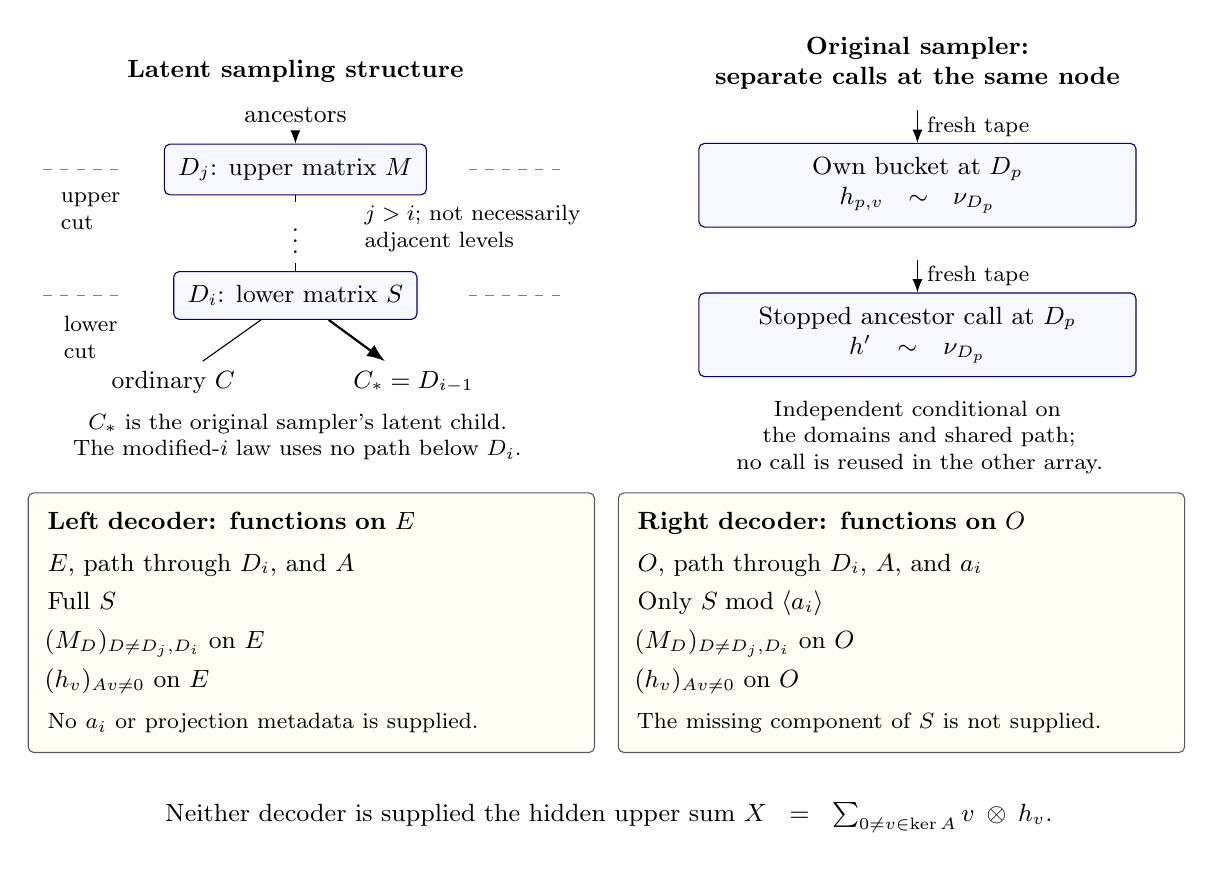
\begin{tikzpicture}[
  >=Latex, font=\small,
  cut/.style={dashed,draw=black!50},
  treebox/.style={draw=blue!45!black,rounded corners=2pt,fill=blue!3,
    align=center,inner sep=5pt},
  inputbox/.style={draw=black!65,rounded corners=2pt,fill=yellow!4,
    align=left,text width=6.7cm,inner sep=7pt}]
\node[font=\small\bfseries] at (3.2,0) {Latent sampling structure};
\node[font=\small\bfseries,align=center] at (11.1,0.1) {Original sampler:\\separate calls at the same node};
\node at (3.2,-0.55) {ancestors};
\node[treebox] (upper) at (3.2,-1.25) {$D_j$: upper matrix $M$};
\draw[->] (3.2,-0.78)--(upper);
\draw[cut] (0,-1.25)--(1.0,-1.25);
\draw[cut] (5.4,-1.25)--(6.6,-1.25);
\node[align=left,font=\footnotesize] at (0.6,-1.78) {upper\\cut};
\node[align=center] (middle) at (3.2,-2.05) {$\vdots$};
\node[align=left,font=\footnotesize] at (5.45,-2.0) {$j>i$; not necessarily\\adjacent levels};
\node[treebox] (lower) at (3.2,-2.85) {$D_i$: lower matrix $S$};
\draw (upper)--(middle);
\draw (middle)--(lower);
\draw[cut] (0,-2.85)--(1.0,-2.85);
\draw[cut] (5.4,-2.85)--(6.6,-2.85);
\node[align=left,font=\footnotesize] at (0.6,-3.38) {lower\\cut};
\node (ordinary) at (1.65,-3.95) {ordinary $C$};
\node (special) at (4.7,-3.95) {$C_* = D_{i-1}$};
\draw (lower)--(ordinary);
\draw[thick,->] (lower)--(special);
\node[align=center,text width=6.5cm,font=\footnotesize] at (3.2,-4.65)
  {$C_*$ is the original sampler's latent child.\\
   The modified-$i$ law uses no path below $D_i$.};
\node[treebox,text width=5.2cm] (own) at (11.1,-1.45)
  {Own bucket at $D_p$\\$h_{p,v}\sim\nu_{D_p}$};
\node[treebox,text width=5.2cm] (call) at (11.1,-3.35)
  {Stopped ancestor call at $D_p$\\$h'\sim\nu_{D_p}$};
\draw[->] (11.1,-0.5)--node[right,font=\footnotesize]
  {fresh tape}(own.north);
\draw[->] (11.1,-2.4)--node[right,font=\footnotesize]
  {fresh tape}(call.north);
\node[align=center,text width=5.8cm,font=\footnotesize] at (11.1,-4.65)
  {Independent conditional on the domains and shared path;\\
   no call is reused in the other array.};
\node[inputbox,anchor=north west] (left) at (-0.2,-5.35) {
  \textbf{Left decoder: functions on $E$}\\[4pt]
  $E$, path through $D_i$, and $A$\\[3pt]
  Full $S$\\[3pt]
  $(M_D)_{D\ne D_j,D_i}$ on $E$\\[3pt]
  $(h_v)_{Av\ne0}$ on $E$\\[4pt]
  \footnotesize No $a_i$ or projection metadata is supplied.
};
\node[inputbox,anchor=north east] (right) at (14.5,-5.35) {
  \textbf{Right decoder: functions on $O$}\\[4pt]
  $O$, path through $D_i$, $A$, and $a_i$\\[3pt]
  Only $S\bmod\langle a_i\rangle$\\[3pt]
  $(M_D)_{D\ne D_j,D_i}$ on $O$\\[3pt]
  $(h_v)_{Av\ne0}$ on $O$\\[4pt]
  \footnotesize The missing component of $S$ is not supplied.
};
\node[fit=(left)(right),inner sep=0pt] (cards) {};
\node[align=center,text width=14cm,below=5mm of cards.south]
  {Neither decoder is supplied the hidden upper sum
   $X=\sum_{0\ne v\in\ker A}v\otimes h_v$.};
\end{tikzpicture}
\caption{Cuts and the information supplied to the decoders.
The selected levels satisfy $j>i$.  The tree depicts latent sampling
choices; the upper-cut comparison forgets the path below $D_j$.
The call panel shows the original sampler; at a modified cut these calls
are replaced by independent uniform draws in the cut space.
An own bucket and a stopped ancestor call at the same node use separate
tapes, independently conditional on the domains and shared path.
The cards summarize the analytical inputs
\eqref{eq:upper-left-input}--\eqref{eq:upper-right-input}, with $W=\ker A$.
The left receives full $S$ without $a_i$; the right receives $a_i$ and
only the quotient of $S$.  Both receive upper buckets with $Av\ne0$ on
their own domains.  These analytical records are distinct from the
original game's canonical partition keys.}
\label{fig:tree-cut}
\end{figure}


For clarity, the independence underlying these inputs is exact, not an
approximation.  Conditional on $O$, the projection choices, and the path
through $D_i$, give each actual node matrix its own random tape.  Give each
scalar bucket in a matrix a fresh recursive call tree, with independent
ordinary-child uniforms and independent factor calls at every product.
All calls that reach $D_i$ terminate in separate uniform draws in
$H_i'$.  In particular, even a call used for an ancestor of $D_j$ and a
bucket of $M$ that both visit $D_j$ use disjoint random tapes.
The product factorization of these tapes implies
\begin{equation}\label{eq:upper-factorization}
 (h_v)_{v\in W\setminus\{0\}}\mathrel{\perp\!\!\!\perp}
 \bigl((h_v)_{v\notin W},(M_D)_{D\ne D_j}\bigr)
 \quad\text{given the domains, path, and }A.
\end{equation}
The same statement remains true if the original questions $E$ and the
projection maps are additionally given: they determine the embeddings of
the spaces but do not change the intrinsic $O$-space sampler.  This also
explains why analytical disclosure of the full $S$ is harmless for this
factorization, although $S$ is not part of the right input.

Let $\mu_{\mathcal R}$ be the distribution on $W\otimes H'$ obtained by
sampling the hidden buckets in \eqref{eq:upper-hidden} with this original
modified-$i$ sampler.  It is a function of the right input alone.  Indeed,
the right knows $O$, the path down to the terminating cut, all spaces and
all sampler parameters.  Independent recursive calls above that cut can
be enumerated on those spaces without knowing $E$, any projection map,
or the missing part of $S$.  Formula~\eqref{eq:upper-factorization} shows
that $\mu_{\mathcal R}$ is also the actual conditional hidden law after
revealing all of the data in both inputs, including full $S$.

For each fixed right input, define
\begin{equation}\label{eq:upper-G}
 G_{\mathcal R}:W\otimes H'\longrightarrow K
\end{equation}
by assembling the level-$i$ right query with upper matrix
$M_{\rm known}+X$, consulting its fixed partition label, and restoring
the upper component.  This is a well-defined local function: the lower
matrix in this query is precisely $S\bmod\langle a_i\rangle$.
The original labeling has already been extended to unused legal keys, so
this definition is total for every $X$ in the ambient space.

Assume that every product count meets the absolute balance minimum of
Lemma~\ref{lem:bias}, and that
\begin{equation}\label{eq:upper-R}
 (7/8)^{R_j}\le\lambda.
\end{equation}
Every nonzero character of $W\otimes H'$ then has bias at most $\lambda$
under $\mu_{\mathcal R}$.  To check this directly, identify a character
with a nonzero linear map $\Phi:W\longrightarrow(H')^*$.  Some nonzero
$v\in W$ has $\Phi(v)\ne0$, so its expectation on the corresponding
bucket has absolute value at most $\lambda$ by Lemma~\ref{lem:bias}.
Independence factors the expectation over all hidden buckets, and all
remaining factors have absolute value at most one.  This argument makes
no claim about small bias after a slice, a successful match, or any later
conditioning.

\subsection{A bounded list for an arbitrary small-bias law}

We record the Fourier calculation separately.  It uses characters under
their actual sampling law rather than treating small bias as total-variation
closeness to uniform measure.  The short-list principle is related to
Goldreich--Levin heavy-character decoding~\cite{GoldreichLevin1989}.
We prove the needed statement for the present nonuniform, own-question law;
no efficient decoding algorithm is required.  If $V=W\otimes H'$, write
\[
 \chi_\Phi(X)=(-1)^{\langle\Phi,X\rangle},\qquad
 \Phi\in V^*=\Hom(W,(H')^*).
\]
For $\sigma\in K^*$ and a fixed function $G:V\longrightarrow K$, put
$g_\sigma(X)=(-1)^{\sigma(G(X))}$.

\begin{lemma}[One heavy list for all affine-slice witnesses]
\label{lem:heavy-list}
Let $K=\F^\ell$, let $W\subseteq K$ have codimension at most $r$, and
let $H'$ be a finite vector space.  Let $\mu$ be a probability law on
$V=W\otimes H'$ with $|\E_\mu\chi_\Phi|\le\lambda$ for every nonzero
$\Phi\in V^*$.  Fix $G:V\longrightarrow K$, $0<\rho\le1$, and set
\[
 h_0=2^{-r\ell},\qquad \tau=\rho h_0/4.
\]
Suppose
\begin{equation}\label{eq:upper-Fourier-conditions}
 2^{-(\ell-r)}<\rho/8,
 \qquad 0\le\lambda\le\min\{h_0/2,\tau^2/2\}.
\end{equation}
For each $\sigma\in K^*$ define the list
\begin{equation}\label{eq:upper-heavy-definition}
 \mathcal H_\sigma
 =\{\Phi\in V^*:|\E_\mu[g_\sigma\chi_\Phi]|\ge\tau\}.
\end{equation}
Each list has size at most $2/\tau^2$.  Moreover, let
$Q\subseteq(H')^*$ have dimension at most $r$, let
$t_Q\in\Hom(Q,W)$ specify the nonempty affine slice
$\mathcal C=\{X:X|_Q=t_Q\}$, and let
$z'\in(H')^*$ and $k_0\in K$.  If
\begin{equation}\label{eq:upper-slice-equality}
 \Prob_\mu(G(X)=Xz'+k_0\mid X\in\mathcal C)\ge\rho,
\end{equation}
then some $\sigma$ with $\sigma|_W\ne0$ has a list element in
\begin{equation}\label{eq:upper-heavy-coset}
 (\sigma|_W)\otimes z'+W^*\otimes Q.
\end{equation}
The lists in \eqref{eq:upper-heavy-definition} depend on $\mu,G,W,H'$ and
$\tau$, and not on the witness $Q,t_Q,z',k_0$.
\end{lemma}

\begin{proof}
Put $w=\dim W$ and $q=\dim Q$.  The map
$V\longrightarrow\Hom(Q,W)$ given by $X\mapsto X|_Q$ is surjective:
choose a basis of $Q$, extend it to a basis of $(H')^*$, and extend any
specified linear map to all of $(H')^*$.  Thus the linear equations for
$\mathcal C$ have rank $wq\le\ell r$.  Their dual space is
$L=W^*\otimes Q\subseteq V^*$.  Choose any $X_0\in\mathcal C$.  The
exact character identity for the affine slice is
\begin{equation}\label{eq:upper-slice-expansion}
 \one_{\mathcal C}(X)
   =\frac1{|L|}\sum_{\Psi\in L}\chi_\Psi(X_0)\chi_\Psi(X).
\end{equation}
Indeed, the sum is one when $X-X_0$ annihilates $L$, and zero otherwise.
Consequently
\begin{equation}\label{eq:upper-slice-mass}
 \mu(\mathcal C)\ge2^{-wq}-\lambda\ge h_0-\lambda\ge h_0/2>0.
\end{equation}
This proves the needed slice mass using unconditional bias.

Expand the equality in \eqref{eq:upper-slice-equality} over $K^*$:
\[
 \Prob_\mu(G(X)=Xz'+k_0\mid\mathcal C)
 =2^{-\ell}\sum_{\sigma\in K^*}(-1)^{\sigma(k_0)}
    \E_\mu[g_\sigma(X)\chi_{(\sigma|_W)\otimes z'}(X)
                    \mid\mathcal C].
\]
The fraction of $\sigma$ annihilating $W$ is $2^{-w}$, which is at most
$2^{-(\ell-r)}<\rho/8$.  Each term has absolute value at most one, so
some remaining $\sigma$ has
\[
 \left|\E_\mu[g_\sigma\chi_{(\sigma|_W)\otimes z'}\mid\mathcal C]\right|
 \ge\rho/2.
\]
Multiply by \eqref{eq:upper-slice-mass} and then insert
\eqref{eq:upper-slice-expansion}.  The coefficients in that expansion
have total absolute value one.  It follows that for some $\Psi\in L$,
\[
 \left|\E_\mu[g_\sigma
       \chi_{(\sigma|_W)\otimes z'+\Psi}]\right|
 \ge(\rho/2)(h_0/2)=\tau.
\]
This gives \eqref{eq:upper-heavy-coset}.  Notice that the unknown target
offset contributes only a sign in the equality expansion.

It remains to bound the lists under the possibly nonuniform law $\mu$.
Take $m$ distinct elements $\Phi_1,\ldots,\Phi_m$ of one list and choose
signs $\epsilon_a\in\{-1,1\}$ aligning their correlations with
$g_\sigma$.  Cauchy--Schwarz gives
\begin{align*}
 m^2\tau^2
 &\le\left(\E_\mu\left[g_\sigma
               \sum_{a=1}^m\epsilon_a\chi_{\Phi_a}\right]\right)^2\\
 &\le\E_\mu\left[\left(\sum_{a=1}^m
                   \epsilon_a\chi_{\Phi_a}\right)^2\right]
 \le m+m(m-1)\lambda\le m+m^2\lambda.
\end{align*}
For distinct indices the product character is nonzero, which justifies
the off-diagonal bound even after sign alignment.  If $m>0$, the hypothesis
$\lambda\le\tau^2/2$ yields $m\le2/\tau^2$; the empty case is immediate.
Only the selected characters were summed, so no ambient-dimension factor
appears.  All correlations defining the lists are unconditional under the
same law $\mu$.
\end{proof}

\subsection{Constructing the two decoders}

\begin{proposition}[Upper decoding with a lower rank test]
\label{prop:upper}
Suppose a legal labeling has acceptance at least $\eps$, $d\eps\ge4$,
and the cut comparisons have the errors required in
\eqref{eq:upper-c}, Lemma~\ref{lem:useful-equality}, and
Lemma~\ref{lem:positive-difference}.  Choose upper inverse constants
$\alpha,r$ and $\ell=\ell_j$ as above, and assume
\eqref{eq:upper-Fourier-conditions} and \eqref{eq:upper-R}, with the
absolute balance minimum at every level.  For the pair $i<j$ supplied by
\eqref{eq:upper-pair}, there are randomized strategies, measurable on
\eqref{eq:upper-left-input} and \eqref{eq:upper-right-input} respectively,
returning bilinear forms $F_L$ on $H_i$ and $F_R$ on $H_i'$ such that
\begin{equation}\label{eq:upper-gamma}
 \Prob_i\bigl(F_R=F_L|_{H_i'\times H_i'}\bigr)\ge
 \gamma_j:=b\,2^{-\ell}\frac{\tau^2}{2}\,2^{-r}>0.
\end{equation}
Every left output has the form
\[
 F_L(x,y)=z(xy),\quad z\in(H_i^2)^*,\quad z(1)=1,
 \qquad \rank\bigl(F_L(S_t,S_u)\bigr)_{t,u}\le1.
\]
The constant $\gamma_j$ depends only on $c,\alpha,r,\ell_j$; it is
independent of the lower row count $\ell_i$, the branching numbers, the
source alphabet and instance size, and the bias accuracies chosen for
lower levels.  The left strategy never receives $a_i$, and the right
strategy uses $S$ only through its quotient by $\langle a_i\rangle$.
\end{proposition}

\begin{proof}
On good advice the left samples $z$ uniformly from $z_0+Z$, using fresh
private randomness, and returns $F_L(x,y)=z(xy)$ for $x,y\in H_i$.
The products belong to $H$ because $D_i$ is a proper descendant of $D_j$.
Equation~\eqref{eq:upper-valid} proves normalization and the rank bound
on $S$.  On bad advice it evaluates at a fixed legal assignment on the
original subtree, obtaining the same two validity properties.  These rules
also define valid defaults on any other well-typed left input: use the
stated construction whenever its witness is valid, and point evaluation
otherwise.  The rule involves no omitted direction.

For the right decoder, use $\mu=\mu_{\mathcal R}$ and
$G=G_{\mathcal R}$ from \eqref{eq:upper-G}, and compute all lists
\eqref{eq:upper-heavy-definition}.  Choose $\sigma\in K^*$ uniformly.
If $\sigma|_W\ne0$ and its list is nonempty, choose an element $\Phi$
uniformly from that list.  Choose $h_\sigma\in W$ deterministically from
$(A,\sigma)$ with $\sigma(h_\sigma)=1$, for example the first such vector
in a fixed order, and put $z_R=\Phi(h_\sigma)\in(H')^*$.  Return
\begin{equation}\label{eq:upper-right-form}
 F_R(x,y)=z_R(xy),\qquad x,y\in H_i'.
\end{equation}
The inclusion $(H_i')^2\subseteq H'$ makes this a bilinear form.  In the
remaining cases return the zero bilinear form.  These defaults make the
algorithm total; normalization is required only of the left output.
No chosen witness from the left enters the right rule.

We now prove agreement for these particular algorithms.  For this analysis
only, expose $E,O$, all projection maps, the path through $D_i$, $A,a_i$,
all nonhidden upper buckets, and all other matrices including full $S$.
Call the resulting data $\mathcal D$.  Do not expose $X$, any hidden
bucket ingredients, the slice event $J$, the representative-match event
$I$, a successful test, or either decoder's final random choices.
This exposure determines $P$, $M_{\rm known}$ and $A\bar M$, since
$AX=0$.  Hence it determines goodness, $Z,z_0,u$ and the column witness.
By \eqref{eq:upper-factorization}, the conditional distribution of $X$
given $\mathcal D$ remains exactly $\mu_{\mathcal R}$, with the bias
bound already proved.

On good data let $Q=Z|_{H'}\subseteq(H')^*$ and $z'=z_0|_{H'}$.
The event $J$ either is impossible, or is an affine slice
\[
 \mathcal C_{\mathcal D}=
 \{X\in W\otimes H':X(q_a|_{H'})=v_a-M_{\rm known}q_a
                         \text{ for every }a\}.
\]
In the latter case these equations define a well-defined linear
specification on $Q$, of dimension at most $r$.  This also handles a
collapse of some columns on restriction to $H'$.  The target in
\eqref{eq:upper-difference} is $Xz'+k_0$, where
$k_0=M_{\rm known}z_0+u$ is fixed by $\mathcal D$.

Set $p_{\mathcal D}=\mu_{\mathcal R}(\mathcal C_{\mathcal D})$ on good
compatible data, and zero otherwise.  When $p_{\mathcal D}>0$, let
\[
 q_{\mathcal D}=
 \Prob_i\bigl(G_{\mathcal R}(X)=Xz'+k_0
                         \mid\mathcal D,\ X\in\mathcal C_{\mathcal D}\bigr),
\]
and set $q_{\mathcal D}=0$ otherwise.  Disintegrating the already proved
unconditional inequality \eqref{eq:upper-difference} gives
\begin{equation}\label{eq:upper-favorable-mass}
 \E_i[p_{\mathcal D}(q_{\mathcal D}-\rho)]\ge b.
\end{equation}
Its integrand is nonpositive unless the data are good and compatible,
$p_{\mathcal D}>0$, and $q_{\mathcal D}\ge\rho$.  The integrand is at
most one everywhere.  The set of data with those properties consequently
has probability at least $b$.  This is the sole use of the finer exposure:
we have not asserted that usefulness persists upon conditioning on it.

Fix any such favorable $\mathcal D$.  Lemma~\ref{lem:heavy-list} supplies
at least one nonannihilating $\sigma$ and one
\[
 \Phi\in\mathcal H_\sigma\cap
       \bigl((\sigma|_W)\otimes z'+W^*\otimes Q\bigr).
\]
The right chooses such a pair with probability at least
$2^{-\ell}\tau^2/2$.  Every such choice, with the already fixed
$h_\sigma$, has
\[
 z_R=\Phi(h_\sigma)\in z'+Q.
\]
The restriction map $Z\longrightarrow Q$ is surjective.  Uniform measure
on $z_0+Z$ therefore pushes to uniform measure on $z'+Q$, so the fresh
left choice has restriction equal to this particular $z_R$ with probability
$2^{-\dim Q}\ge2^{-r}$.  It is independent of the right's final choices
conditional on $\mathcal D$.  Equality of these functionals on $H'$
implies agreement of their product forms on $H_i'\times H_i'$.
Averaging over the favorable data proves \eqref{eq:upper-gamma}.

For a fixed right input, the law $\mu_{\mathcal R}$, function
$G_{\mathcal R}$, lists $\mathcal H_\sigma$, and contraction vectors
$h_\sigma$ are identical for all compatible left inputs and witnesses.
Different favorable exposures may certify different elements of these same
lists.  The preceding hit probability holds separately for each exposure,
so averaging introduces no factor for the number of witnesses.

Finally, $\eta,\alpha,r$ were fixed from $c$, while $g,q_0,b,\rho,\tau$
were fixed from these constants and $\ell_j$.  Conditions
\eqref{eq:upper-Fourier-conditions} require only an upper row-count
lower bound and an upper bias tolerance.  Condition~\eqref{eq:upper-R}
is met by choosing $R_j$ large enough; below $j$ it uses only the common
absolute balance minimum.  The inverse statement applies to $H/B$ even
in small dimension by Lemma~\ref{lem:padding}.  Thus none of these choices
depends on the later lower row count or source and branching dimensions.
\end{proof}

The algorithms in Proposition~\ref{prop:upper} are now fixed local rules.
In particular, the right rule always computes its heavy lists from the
original law $\mu_{\mathcal R}$ just defined.  A later conditioning may
change the physical law of the hidden buckets; it does not change that
algorithm.  The subsequent rank and repetition arguments use these same
rules with their prescribed inputs.

\section{From tested rank to full rank}\label{sec:lower}

Proposition~\ref{prop:upper} provides two local decoders whose bilinear
forms agree after projection with probability at least $\gamma_j>0$.
The left form has rank at most one on the displayed lower rows.  We now
show that a positive part of this agreement comes from left forms of
bounded rank on the entire lower function space.  The distinction matters:
the form selected by the decoder can depend on the rows on which it is
tested.

The passage from agreement of restricted forms to a fixed form of bounded
rank has a close predecessor in Fei, Minzer and Wang
\cite[Lemmas~5.15--5.16]{FeiMinzerWang2026}.  Here we carry it out for the
tree function spaces, using the sparse-projection posterior bound and
an estimate on affine row and column slices.

Fix the levels $i<j$, and write
\[
 H_i=H_{D_i}(E),\qquad H_i'=H_{D_i}(O)\subseteq H_i,
 \qquad K_i=\F^{\ell_i},\qquad S=M_{D_i}.
\]
All restrictions below use the injective pullback identifying $H_i'$ with
a subspace of $H_i$.  For a bilinear form $F$ on $H_i$, let
\[
 \operatorname{Gram}_F(S)
       =\bigl(F(S_u,S_v)\bigr)_{1\leq u,v\leq\ell_i}.
\]
Call $F$ \emph{admissible at $S$} if there is a linear functional
$z\in(H_i^2)^*$ such that
\begin{equation}\label{eq:lower-admissible}
 F(x,y)=z(xy),\qquad z(1)=1,\qquad
 \rank\operatorname{Gram}_F(S)\leq1.
\end{equation}
The left form in Proposition~\ref{prop:upper} is admissible: its functional
on $H_{D_j}(E)$ restricts to $H_i^2$, since $D_i$ is a proper descendant
of $D_j$.  On a default input a legal point evaluation has the same
properties.  Admissibility is a condition on the left input and output
alone; in these finite spaces it can also be checked by solving the
linear equations for $z$ and computing a matrix rank.

\subsection{Local tapes and the unfiltered pair experiment}

We first specify the randomness to be used without enlarging either
decoder's information.  At the modified cut at $D_i$, condition on
$E,O$, the projections and the path through $D_i$.  The advice outside the
list $S$ is generated by independent exterior ingredients, independent
uniform descendant arrays in their projected spaces, and a bounded
number of independent uniform scalar calls in $H_i'$.  The scalar calls
generate all dependencies of ancestor arrays and the visible level-$j$
buckets.  The list $S$ uses fresh randomness independent of all these
calls.  This uses the stopped-call representation of
Lemma~\ref{lem:stopped-calls}, with the independent cut rows in the modified
experiment defined before Lemma~\ref{lem:sparse-tv}.  In particular, already assembled ancestor arrays
are functions of these calls and the exterior ingredients; they are not
additional independent exterior variables.

The direct-row representation in Equation~\eqref{eq:direct-cut-count}
uses $\widehat T_i$ scalar cut rows, including the rows of $S$.
The lower resampling below adds one independent row, giving the count
$\widehat T_i+1$ for that comparison.
Calls may be included before the row map $A$ selects which level-$j$
buckets are visible.  Thus their number depends on the fixed row and
product counts, and not on $n_i$ or on branching at higher levels.

The left decoder receives $E$, the path through $D_i$, its displayed
arrays including $S$, the upper row map $A$, and the prescribed visible
upper buckets as functions on its own domains.  It receives neither
$O$, the projection choices, nor the omitted lower direction $a_i$.
The right decoder receives its corresponding data on $O$, together with
$a_i$ and $S\bmod a_i$, and receives no ingredients determining the
missing part of $S$.  The latent data just described are an analytical
representation of these inputs, not additional inputs to the decoders.

A \emph{complete local random tape} specifies the decoder's random
choices on every possible local input.  Since all input and output sets
are finite, each randomized decoder is a distribution on deterministic
local functions.  Averaging therefore permits fixing both complete
tapes while preserving any hypothesized unconditional agreement
probability.  Such a fixing does not condition on a realized answer or
on an agreement event.  For a cutoff $s$, erase a left output if it is
not admissible at its own input or if its full rank is at most $s$.
This erasure depends only on the left input and its fixed tape.

\begin{lemma}[Resampling and transfer to full equality]\label{lem:resampling}
Fix complete local tapes and the left erasure just described.  Suppose
the nonerased left form agrees with the right form on $H_i'\times H_i'$
with probability $h$ in the modified experiment.  Let $L_i$ be a
simultaneous child likelihood bound for the lifted raw cut data,
including the rows of $S$ and one additional independent row.  Let
$\upsilon_i$ bound the total variation between these lifted data and
their unrestricted uniform version.  There is an unrestricted
experiment in which $S\in K_i\otimes H_i$ and $l\in H_i$ are independent
uniform variables, $a_i\in K_i\setminus\{0\}$ is uniform and independent,
and
\begin{equation}\label{eq:lower-full-equality}
 \Pr_{\mathrm{unif}}\bigl[
 f(S)=f(S+a_i l)\ne\bot\bigr]
 \geq h^2-\frac{2\beta_i L_i}{1-\beta_i}-\upsilon_i.
\end{equation}
Here $f$ also depends on background data independent of $(S,a_i,l)$
conditional on the domains.  For every fixing of that background it is
one partial table on $K_i\otimes H_i$, with no $a_i$ or $l$ input.  Every
defined output is admissible at its argument and has full rank greater
than $s$.
\end{lemma}

\begin{proof}
We use two disintegrations of the same pair distribution.  The first
establishes a lower bound for agreement of restrictions; the second
bounds the chance that unequal full forms become equal after projection.

For the first disintegration, let $\mathcal C$ include both domains,
all projections, the path through $D_i$, $A$, exterior ingredients,
descendant arrays, and all cut calls other than those generating $S$.
The fixed tapes are part of this background.  Conditional on
$(\mathcal C,a_i)$, the list $S$ is uniform in $K_i\otimes H_i'$.
Write $q=S\bmod a_i$.  Once $(\mathcal C,a_i,q)$ is fixed, the right
input and hence its answer $F_R$ are fixed.  Let
\[
 p(\mathcal C,a_i,q)=
 \Pr\bigl[f(S)\ne\bot,
       \ f(S)|_{H_i'\times H_i'}=F_R
          \mid\mathcal C,a_i,q\bigr].
\]
Draw $S,S'$ independently from this same quotient fiber.  Conditional
independence and then Cauchy--Schwarz give
\begin{equation}\label{eq:lower-fiber-square}
 \Pr[\text{both draws agree with }F_R\text{ and are nonerased}]
   =\E[p^2]\geq(\E p)^2=h^2.
\end{equation}
In particular both defined left restrictions agree with each other
with probability at least $h^2$.

Before either agreement event is inspected, this pair distribution has
the following exact alternative description:
\begin{equation}\label{eq:lower-unfiltered-law}
 \begin{gathered}
 \mathcal C\text{ has its original law},\qquad
 a_i\text{ is uniform nonzero},\\
 S\text{ is uniform in }K_i\otimes H_i',\qquad
 l\text{ is independently uniform in }H_i',\\
 S'=S+a_i l.
 \end{gathered}
\end{equation}
Indeed the quotient $q$ has its original marginal, the first draw is
uniform, and for every fixed $S$ the map
$l\mapsto S+a_i l$ is a bijection from $H_i'$ onto the fiber containing
$S$.  Thus the pair construction has introduced no filtering by either
success or rank.  The inequality in Equation~\ref{eq:lower-fiber-square}
is an event probability under the unfiltered law
\eqref{eq:lower-unfiltered-law}.

For the second disintegration, expose $E$, the independent exterior
ingredients, the path through $D_i$, $A$, the fixed tapes, and $a_i$.
Within each child of $D_i$, expose only the \emph{lifted raw block}:
the child summands for all cut calls, including the rows of $S$ and
$l$, and its descendant arrays.  Do not expose $O$, projection metadata,
the right answer, or any success event.  Let $\mathcal D$ denote this
exposure.  All visible left inputs for both draws are functions of
$\mathcal D$.  Consequently both full left outputs are determined by
$\mathcal D$, even though the projection flags need not be.

Write $F_0=f(S)$ and $F_1=f(S+a_i l)$.  On inputs where either value
is undefined, assign that output the zero bilinear form solely for applying
Lemma~\ref{lem:posterior}.  The resulting two forms are functions of the
permitted lifted data $\mathcal D$.  That lemma applies with the enlarged
call family containing the extra row $l$: the exposure includes the
independent direction and fixed tapes, but no projection metadata or right
response.  Its bilinear consequence~\eqref{eq:adaptive-bilinear-error}
therefore gives
\begin{equation}\label{eq:lower-bad-restriction}
 \Pr\bigl[F_0,F_1\ne\bot,\ F_0\ne F_1,
                   \ F_0|_{H_i'\times H_i'}=F_1|_{H_i'\times H_i'}\bigr]
       \leq\frac{2\beta_i L_i}{1-\beta_i}.
\end{equation}
Here $F_0,F_1\ne\bot$ refers to the original partial-table outputs.
The inequality is unconditional under the pair law
\eqref{eq:lower-unfiltered-law}; neither successful draw has been used
as a conditioning event.  Subtracting
Equation~\ref{eq:lower-bad-restriction} from the event probability in
Equation~\ref{eq:lower-fiber-square} yields full defined equality with
probability at least $h^2-2\beta_i L_i/(1-\beta_i)$.

Full defined equality depends only on $E$, the lifted raw data and the
independent exterior choices.  Lemma~\ref{lem:sparse-tv}, applied with
the extra row $l$, therefore transfers this event at loss at most
$\upsilon_i$ to the unrestricted cut law.  In that law $S,l$ are fresh
independent uniforms on $H_i$, all other cut calls and descendant
arrays are independent of them, and $a_i$ is independent of all these
data.  This proves Equation~\ref{eq:lower-full-equality}.

For clarity, the function evaluated at an arbitrary unrestricted input
$S$ is the original left algorithm on its reconstructed input, followed
by the local erasure.  In particular, its space $B=B(S)$, splitting of
$H_{D_j}(E)/B(S)$, good-advice predicate and chosen upper slice witness
are recomputed from that input.  The usefulness marks and witness
selection \emph{rules} remain the fixed rules of
Section~\ref{sec:upper}; their values are not held constant as $S$
varies.  Neither $a_i$ nor $l$ is passed to this algorithm.  Values
outside the original support are defined by the same local extension
and erased if they fail \eqref{eq:lower-admissible}.  Fixing the other
independently generated data therefore leaves a single partial table
$f(S)$ with all the asserted pointwise properties.
\end{proof}

We have converted substantial high-rank agreement into equality of one
partial table under an ordinary rank-one step.  The inverse theorem
will select a single output form dense on a row/column slice.  The next
lemma shows that a fixed form of high rank cannot pass the tested rank
condition on such a slice, even when its free rows have affine offsets.

\subsection{A rank bound on affine slices}

\begin{lemma}[Fixed forms on affine row/column slices]\label{lem:rank-slice}
Let $H$ be a finite-dimensional vector space over $\F$, let $F$ be a
bilinear form on $H$, and let $\ell,r',m$ be nonnegative integers with
$m\geq1$ and $\ell\geq2m+r'$.  Let $\mathcal A\subseteq H^\ell$ be a
nonempty affine slice defined by at most $r'$ row combinations and at
most $r'$ column functionals: for suitable linear maps $A_0$ and
$q_1,\ldots,q_b\in H^*$, where $b\leq r'$,
\[
 \mathcal A=\{S:A_0S=U,\ S q_v=w_v\ (1\leq v\leq b)\},
 \qquad A_0\text{ has at most }r'\text{ rows}.
\]
Then, for uniform $S\in\mathcal A$ and $t_0=\rank F-2r'$,
\begin{equation}\label{eq:lower-rank-slice-bound}
 \Pr\bigl[\rank\operatorname{Gram}_F(S)\leq1\bigr]
 \leq (2^m-1)2^{-t_0}
       +\bigl[1+(2^m-1)^2\bigr]2^{-m^2}.
\end{equation}
In particular, if $\rank F>s$, the first term can be replaced by
$2^{m-(s-2r')}$.
\end{lemma}

\begin{proof}
The form $F$ is fixed throughout this proof.  First remove dependent
row equations, leaving $a=\rank A_0\leq r'$ independent ones.
Nonemptiness of the slice guarantees the corresponding relations among
their prescribed values.  Extend these $a$ row combinations to an
invertible matrix $T\in\Mat_{\ell\times\ell}(\F)$ and put $Y=TS$.
The first $a$ rows of $Y$ are fixed.  Bilinearity gives the congruence
\begin{equation}\label{eq:lower-gram-congruence}
 \operatorname{Gram}_F(Y)
       =T\operatorname{Gram}_F(S)T^{\mathsf t}.
\end{equation}
It follows that the two Gram matrices have the same rank.  We are
transforming the rows of a fixed form, and make no equivariance
assumption about any decoder that might have selected $F$.

Remove dependent column functionals as well, leaving a basis
$q_1,\ldots,q_c$ of their span with $c\leq r'$.  Again, the nonempty
slice guarantees every required dependence among the right-hand sides.
The column equations transform to $Yq_v=Tw_v$.  Define
\[
 N=\bigcap_{v=1}^c\ker q_v,\qquad \operatorname{codim}_H N=c.
\]
After the first $a$ rows have been fixed, the equations on each remaining
row are independent of those on the other rows and specify a nonempty
translate of $N$.  Thus the uniform slice measure makes its
$\ell-a\geq2m$ free rows independent, each uniform on a possibly
different affine space $u_k+N$.  This conclusion also covers redundant
original equations, zero column span, and zero row rank.

Let $F_N$ be the restriction of $F$ to $N\times N$, and put
$t=\rank F_N$.  Regard a bilinear form as a map from its first argument
space to the dual of its second argument space.  Restricting the
domain from $H$ to $N$ loses at most $c$ in rank.  Restricting the
codomain from $H^*$ to $N^*$ also loses at most $c$, since the restriction
map has a kernel of dimension $c$.  Consequently
\begin{equation}\label{eq:lower-rank-loss}
 t\geq\rank F-2c\geq\rank F-2r'=t_0.
\end{equation}

Choose two disjoint groups of $m$ free rows, denoted
$x_1,\ldots,x_m$ and $y_1,\ldots,y_m$.  Write
$x_u=u_u+n_u$ with independent uniform $n_u\in N$.  The full
functionals supplied by the first group are
\[
 \lambda_u=F(x_u,\cdot)|_N
     =F(u_u,\cdot)|_N+F(n_u,\cdot)|_N\in N^*.
\]
Let $V\subseteq N^*$ be the image of $F_N$, of dimension $t$.
Each $\lambda_u$ is uniform on its specified translate of $V$, and the
$\lambda_u$ are independent.  For any nonzero
$e=(e_1,\ldots,e_m)\in\F^m$, the sum
$\sum_u e_u\lambda_u$ is uniform on a translate of $V$: select one
index with $e_u=1$ and condition on all other summands.  Its probability
of being zero is therefore either zero or $2^{-t}$.  Taking the union
over the $2^m-1$ nonzero coefficient vectors gives
\begin{equation}\label{eq:lower-affine-dependence}
 \Pr[\lambda_1,\ldots,\lambda_m\text{ are linearly dependent}]
       \leq(2^m-1)2^{-t}.
\end{equation}
The offsets $F(u_u,\cdot)|_N$ are included in these functionals; no
claim about independence of only their variable parts is being made.

Conditional on a realization of the first group for which the
$\lambda_u$ are linearly independent, the linear map
\[
 N\longrightarrow\F^m,\qquad
 n\longmapsto(\lambda_1(n),\ldots,\lambda_m(n))
\]
is surjective.  A second-group row $y_v=v_v+n_v'$ has $n_v'$ uniform
in $N$, independently of the first group and of the other such rows.
Its cross column $(F(x_u,y_v))_{u=1}^m$ is a fixed offset plus the image
of $n_v'$ under this surjection.  It is therefore uniform in $\F^m$.
The cross matrix
\[
 C=\bigl(F(x_u,y_v)\bigr)_{1\leq u,v\leq m}
\]
is consequently uniform in $\Mat_{m\times m}(\F)$, conditional on that
first group.

Exactly one such matrix has rank zero.  Every rank-one matrix has a
factorization $uv^{\mathsf t}$ with nonzero $u,v\in\F^m$, unique over
$\F$ because the only nonzero scalar is one.  Hence exactly
$1+(2^m-1)^2$ matrices have rank at most one.  If the full Gram matrix
of $Y$ has rank at most one, its cross submatrix $C$ does as well.
Combining this count with
Equations~\ref{eq:lower-gram-congruence},
\ref{eq:lower-rank-loss} and~\ref{eq:lower-affine-dependence} proves
\eqref{eq:lower-rank-slice-bound}.  Finally, $\rank F>s$ implies
$(2^m-1)2^{-t}\leq2^{m-(s-2r')}$, giving the stated simpler bound.
Neither symmetry nor nonalternation of $F$ was required.
\end{proof}

\subsection{Positive agreement of bounded-rank forms}

\begin{proposition}[Low-rank agreement]\label{prop:low-rank}
Fix a pair $i<j$ for which Proposition~\ref{prop:upper} supplies
agreement at least $\gamma=\gamma_j>0$.  Apply
Theorem~\ref{thm:inverse}, including Lemma~\ref{lem:padding}, at the
equality threshold
\[
 \eta_{\mathrm{low}}=\gamma^2/8,
\]
and let $\alpha'>0$, $r'$ and $\ell_0'$ be its density, constraint and
row-count constants.  Choose integers $m\geq1$, $s\geq1$ and $\ell_i$
such that
\begin{equation}\label{eq:lower-parameter-conditions}
 \bigl[1+(2^m-1)^2\bigr]2^{-m^2}<\alpha'/2,
 \qquad 2^{m-(s-2r')}<\alpha'/2,
 \qquad \ell_i\geq\max\{\ell_0',2m+r'\}.
\end{equation}
Take $n_i$ sufficiently large that the data in
Lemma~\ref{lem:resampling} satisfy
\begin{equation}\label{eq:lower-error-conditions}
 \frac{2\beta_iL_i}{1-\beta_i}\leq\gamma^2/64,
 \qquad \upsilon_i\leq\gamma^2/64,
 \qquad \beta_i=n_i^{-2/3}.
\end{equation}
Then the original randomized decoders satisfy, in the modified
experiment,
\begin{equation}\label{eq:lower-low-rank-mass}
 \Pr\bigl[F_L|_{H_i'\times H_i'}=F_R,
       \ F_L\text{ is admissible at }S,
       \ \rank F_L\leq s\bigr]\geq\gamma/2.
\end{equation}
The rank cutoff and row-count requirements depend only on the upper
agreement constant.  The likelihood and total-variation requirements
can be met after the source alphabet and lower branching numbers have
been fixed, without any dependence on higher branching numbers.
\end{proposition}

\begin{proof}
Suppose instead that agreement from left outputs of rank greater than
$s$ has probability at least $\gamma/2$.  Fix complete local tapes
preserving this high-rank agreement mass, and erase the left outputs
as above.  Since the original left decoder is admissible, this leaves
nonerased agreement probability $h\geq\gamma/2$.  By
Lemma~\ref{lem:resampling} and
Equation~\ref{eq:lower-error-conditions}, the unrestricted experiment
satisfies
\[
 \Pr_{\mathrm{unif}}[f(S)=f(S+a_i l)\ne\bot]
 \geq\frac{\gamma^2}{4}-\frac{\gamma^2}{64}
                         -\frac{\gamma^2}{64}
 =\frac{7\gamma^2}{32}>\eta_{\mathrm{low}}.
\]
Fix the domains and all remaining independent background data at a
value for which this equality probability is at least
$\eta_{\mathrm{low}}$.  Conditional on this fixing, $S,l,a_i$ still
have the independent uniform laws required by the inverse theorem.
The output alphabet is the finite set of bilinear forms on this fixed
$H_i$; its size has no effect on the inverse constants.

Theorem~\ref{thm:inverse} now selects one \emph{fixed} defined output
$F$ and a nonempty affine row/column slice, with at most $r'$ constraints
of either type, on which $f(S)=F$ has density at least $\alpha'$.
Every such occurrence satisfies $\rank F>s$ and
$\rank\operatorname{Gram}_F(S)\leq1$, by the pointwise definition of
the partial table.  Only after fixing this output do we apply the row
operations in Lemma~\ref{lem:rank-slice}.  That lemma and
Equation~\ref{eq:lower-parameter-conditions} show that the latter
rank event has density strictly less than $\alpha'$ on the same slice,
a contradiction.  Dependence of $B(S)$ and the upper witness on $S$
does not enter this step: at each occurrence of the selected form its
Gram rank condition holds on that occurrence's own list.

Thus high-rank agreement has probability less than $\gamma/2$ for the
original randomized decoders.  Subtracting it from the agreement mass
at least $\gamma$ proves Equation~\ref{eq:lower-low-rank-mass}.  The
temporary fixing of tapes was used only to refute the hypothesized
high-rank mass; it has not replaced the original decoder algorithms
in the conclusion.

For the parameter claims, the second summand in
Equation~\ref{eq:lower-rank-slice-bound} tends to zero as $m$ grows.
Choose $m$ first, then $s$, and then $\ell_i$ as in
\eqref{eq:lower-parameter-conditions}.  All these choices depend only
on $\gamma$.  The finite likelihood bound $L_i$ is fixed once the
source alphabet, upper row and product counts, and lower branching
numbers have been fixed; the extra resampling row changes only this
finite bound.  Lemmas~\ref{lem:sparse-tv} and~\ref{lem:posterior} then
make both losses in \eqref{eq:lower-error-conditions} arbitrarily small
by increasing $n_i$.  For the finitely many upper levels $j>i$, one
may meet all row requirements and take the maximum rank cutoff.
Increasing a cutoff only strengthens every high-rank exclusion already
proved.
\end{proof}

The resulting agreement event supplies a normalized product form of
bounded full rank.  Its restrictions to the atomic indicators at a
leaf will produce an odd list of at most $s$ legal answers.  The next
section turns those lists into local strategies on many independent
source questions.

\section{Clean children and independent repetition}
\label{sec:clean}

A normalized product form of bounded rank determines a short odd list
of answers at each source leaf.  When the decoded forms agree after
projection, their lists satisfy a projection constraint.  To apply
parallel repetition to these lists, we must recover independent source
edges and local answer rules despite their sampled advice.

We do this by finding projected children whose contributions to every
sampled function are zero.  The probability of this event is exactly
independent of their source questions.  Revealing the remaining data
therefore leaves independent source edges at designated leaves, and
each player can reconstruct its original decoder input from its own
questions there.  Repetition then bounds the low-rank agreement from
Proposition~\ref{prop:low-rank}.

Fix levels $i<j$ and use the modified experiment at $D_i$ throughout
this section.  Write
\[
 H_i=H_{D_i}(E),\qquad H_i'=H_{D_i}(O),\qquad S=M_{D_i}.
\]
We identify $H_i'$ with its pullback subspace of $H_i$.  The integer
$s\ge1$ is a full-rank cutoff as in
Proposition~\ref{prop:low-rank}.  The source game, denoted by
$G_{\mathrm{src}}$, is a fixed $t$-fold power of the clause--variable
game.  For a source question $u$ on the left and $v$ on the right,
write $\Lambda_u$ and $\Gamma_v$ for their nonempty legal answer sets.
Thus $\Gamma_v=\F^t$, with a separate coordinate for each slot,
including slots with repeated variable IDs.  Let $\mu$ be the
distribution on source edge records $e=(u,v,\pi_e)$.

\subsection{Odd lists and leaf indicators}

For a finite nonempty set $\Lambda$, define
\[
 \mathcal O_s(\Lambda)
 =\{L\subseteq\Lambda:1\le |L|\le s, |L|\text{ odd}\}.
\]
Given a map $\pi:\Lambda\to\Gamma$, define its parity pushforward by
\begin{equation}
 \pi_{\mathrm{odd}}(L)
 =\{b\in\Gamma:|L\cap\pi^{-1}(b)|\text{ is odd}\}.
 \label{eq:clean-parity-map}
\end{equation}
The same parity pushforward describes restriction of Fourier characters
in low-degree long-code analysis
\cite[Section~2.3, Equation~(1), ECCC version]{DinurGuruswami2015}.
The odd-list game $G_{\mathrm{odd},s}$ has the same questions and edge
distribution as $G_{\mathrm{src}}$, legal answers
$\mathcal O_s(\Lambda_u)$ and $\mathcal O_s(\Gamma_v)$, and edge map
$(\pi_e)_{\mathrm{odd}}$.

\begin{lemma}[Odd-list projection and extraction]
\label{lem:parity-game}
Every map in Equation~\eqref{eq:clean-parity-map} sends
$\mathcal O_s(\Lambda)$ into $\mathcal O_s(\Gamma)$.  In particular,
$G_{\mathrm{odd},s}$ is a total projection game, and
\begin{equation}
 \val(G_{\mathrm{odd},s})\le s^2\val(G_{\mathrm{src}}).
 \label{eq:clean-list-value}
\end{equation}
Suppose a bilinear form $F$ on $H_i$ has the form
\[
 F(x,y)=z(xy),\qquad z\in(H_i^2)^*,\qquad z(1)=1,
 \qquad \rank F\le s.
\]
For every leaf $\lambda$ below $D_i$, with local answer set
$\Lambda_\lambda$, its diagonal on the leaf indicators specifies a
member of $\mathcal O_s(\Lambda_\lambda)$.  If that leaf is projected
by $\pi_e$ and a form $F'$ on $H_i'$ equals the restriction of $F$,
then its corresponding diagonal list is the parity pushforward of
the left list.
\end{lemma}

\begin{proof}
For $L\in\mathcal O_s(\Lambda)$, summing all preimage multiplicities
modulo two gives
\[
 |\pi_{\mathrm{odd}}(L)|\equiv |L|\equiv1\pmod2.
\]
Each member of $\pi_{\mathrm{odd}}(L)$ has at least one preimage in
$L$, and these preimage sets are disjoint.  Consequently its size is
at most $|L|$, proving totality.

Take any deterministic labeling of the odd-list game.  Each player
independently chooses a uniformly random member of the list it would
return.  On an accepted list edge, the two lists contain an accepting
ordinary answer pair: any element of the nonempty right list has an
odd, hence positive, number of preimages in the left list.  The
independent choices select some accepting pair with probability at
least $1/(|L||R|)\ge s^{-2}$.  This is a legal randomized source
strategy; averaging deterministic answer tables bounds its success
by $\val(G_{\mathrm{src}})$.  Maximizing over the list labeling proves
Equation~\eqref{eq:clean-list-value}.

For the extraction statement, let $e_a$ be the indicator that the
answer at leaf $\lambda$ is $a\in\Lambda_\lambda$, extended by
ignoring every other leaf.  By Definition~\ref{def:spaces},
$e_a\in H_i$.  Pointwise multiplication gives
\[
 e_ae_b=0\quad(a\ne b),\qquad e_a^2=e_a,
 \qquad \sum_{a\in\Lambda_\lambda}e_a=1.
\]
Thus $(F(e_a,e_b))_{a,b}$ is diagonal, with diagonal
$d_a=z(e_a)$.  Its rank is the integer $|\{a:d_a=1\}|$ and is at
most $\rank F\le s$.  Moreover,
$\sum_a d_a=z(1)=1$ in $\F$, so this support is odd and nonempty.

For a projected answer $b$, the pullback of its indicator is
\[
 e_b'=\sum_{a:\pi_e(a)=b}e_a.
\]
Agreement of the forms and the diagonal identity imply
\begin{equation}
 F'(e_b',e_b')
 =\sum_{a:\pi_e(a)=b}d_a.
 \label{eq:clean-indicator-pushforward}
\end{equation}
The support on the right is exactly the parity pushforward in
Equation~\eqref{eq:clean-parity-map}, completing the proof.
\end{proof}

Low-rank symmetric matrices also yield short assignment lists in the
quadratic-code analysis of Khot and Saket, through rank-one decompositions
\cite[Lemma~2.1 and Section~7.2, ECCC version]{KhotSaket2017}.
Here the orthogonal leaf indicators give the lists directly as diagonal
supports of legal answers.

We use a total local extraction rule also when a decoder fails to
return such a form.  Order the legal answers to every source question
once and for all.  At each designated leaf, a player reads the
diagonal support of its own output form.  If that support is odd and
has size at most $s$, it returns the support.  If the output is not a
form or this test fails, it returns the singleton consisting of the
first legal answer to its own question.  The test and default use
only that player's input and output.  In particular, the right
player need not determine the rank or validity of the left form.
These rules produce legal lists on every input, and Lemma~\ref{lem:parity-game}
identifies their outputs whenever normalized low-rank agreement occurs.

\subsection{An exact law for vanishing advice}

Zero advice was already used to hide a source coordinate and recover
soundness under repetition by Khot, Minzer and Safra
\cite[Sections~3.3--3.4, especially Remark~3.2]{KhotMinzerSafra2017}.
Here we zero all sampled contributions from selected children and prove
that the resulting conditional source law is exactly a product law.

Choose the first leaf of each child of $D_i$ as its designated leaf.
This choice depends only on the ordered tree.  We will express every
uniform cut draw as a sum of independent child contributions.  A projected
child will be clean when all its contributions and all its internal arrays
are zero.  Its arguments then disappear from the sampled functions, while
the zero probability can be computed on that child's projected domain.

The family of contributions must cover every input used by the decoders.
Stop every recursive scalar call used by an ancestor array when it first
reaches $D_i$, including the calls for every bucket of $M=M_{D_j}$.
Fix this family before the row map $A$ selects visible buckets, and add
the $\ell_i$ independent rows of the uniform matrix $S$.
By Equation~\eqref{eq:direct-cut-count}, its size is
\begin{equation}
 T_i^{\mathrm{cl}}=\widehat T_i=\ell_i+
 \sum_{h=i+1}^{d}(2^{\ell_h}-1)
                   \prod_{p=i+1}^{h}(2R_p).
 \label{eq:clean-call-count}
\end{equation}
Indeed, an array at level $h$ has $2^{\ell_h}-1$ scalar buckets, and
each scalar call at level $p>i$ makes $2R_p$ calls in its path child.
All other contributions lie outside $D_i$, and distinct calls use fresh
randomness.  If a recipe uses fewer calls, pad it with independent unused
calls to reach $T_i^{\mathrm{cl}}$.  Thus the call count is fixed before any
visibility decision.  The notation $T_i^{\mathrm{cl}}$ distinguishes this
family from those enlarged by extra rows in comparison experiments.

Let $\Xi$ record the questions outside $D_i$, the path through $D_i$,
the exterior ingredients of the stopped expressions, and all other arrays
supported outside $D_i$.  Include the independent choices $A$ and $a_i$
after fixing the call family.  Record each exterior function on the domain
of its supporting subtree, together with its location in the expression.
This representation requires no endpoint questions inside $D_i$; each
player will later extend it to its own product domain by ignoring the
other arguments.  Assembled ancestor values are still functions of the
pending cut calls and are not exposed in $\Xi$.
Consequently $\Xi$ depends only on exterior source records and independent
exterior randomness, so the source samples inside $D_i$ retain their
independent laws conditional on $\Xi$.

It is convenient to sample a complete source edge at every leaf,
even when its child will remain unprojected.  This merely augments
the modified experiment: sample the left question and then a source
projection conditional on it, using that projection only if the
child is selected.  For each child $C$ of $D_i$, independently let
$P_C$ be its projection flag, with
$\Pr(P_C=1)=\beta_i=n_i^{-2/3}$.  Write $\boldsymbol e_C$ for the
tuple of source edge records at its leaves and $m_i$ for the number
of those leaves.  Thus $\boldsymbol e_C$ has distribution
$\mu^{\otimes m_i}$.

Generate cut call $q\in[T_i^{\mathrm{cl}}]$ by taking, independently for all
$q,C$, a uniform latent summand
\[
 U_{q,C}\in H_C(O)^2,
 \qquad U_q=\sum_{C\text{ child of }D_i}U_{q,C}.
\]
The sum is uniform in $H_i'$ because the addition map from the
product of the child square spaces onto $H_i'$ is a surjective linear
map.  Its fibers all have the same size.  The resulting calls are
independent, and are independent of the uniform arrays at every
nonleaf proper descendant of $D_i$.  The first $\ell_i$ calls can
therefore serve as the rows of $S$, with the rest substituted in the
stopped ancestor expressions.  This is exactly the modified sampling
law on the visible arrays.  No direct-sum assumption on the child
spaces is involved.

Call $C$ \emph{clean} if $P_C=1$, every $U_{q,C}$ is zero, and every
sampled array at a nonleaf node in the subtree rooted at $C$ is zero.
Write $\mathcal C$ for the set of clean children.

\begin{lemma}[Exact clean probability and conditional source law]
\label{lem:clean-law}
Conditional on any exterior datum $\Xi=\xi$ of positive probability,
the clean indicators are independent.  In the padded construction
above each has probability $\beta_i p_{0,i}$, where
\begin{equation}
 p_{0,i}=
 2^{-T_i^{\mathrm{cl}}\dim(H_C'^2)
       -\displaystyle\sum_{\substack{D\preceq C\\D\text{ nonleaf}}}
           \ell_{\operatorname{level}(D)}\dim H_D'}>0.
 \label{eq:clean-zero-probability}
\end{equation}
Here $D\preceq C$ includes $D=C$, and $H_D'$ is the function space
on a fully projected subtree of the indicated shape.  The exponent
has the same value for every child and every choice of source
questions and projection positions.  It depends only on the source
power, the fixed row and product counts, and branching below level
$i$; it is independent of the instance, $n_i$, and all higher
branching numbers.

After fixing $\mathcal C$, expose all source questions, projection
choices and latent data at nonclean children, and all source edge
records at nondesignated leaves of clean children.  Denote this
additional exposure together with $\Xi$ and $\mathcal C$ by
$\mathcal D_{\mathrm{pub}}$.  Conditional on every value of $\mathcal D_{\mathrm{pub}}$ of positive
probability, the source edge records at the designated clean leaves
are independent and each has distribution $\mu$.
\end{lemma}

\begin{proof}
Fix $\Xi=\xi$ and a child edge tuple $\boldsymbol e_C$.  Conditional
on $P_C=1$, the $T_i^{\mathrm{cl}}$ latent summands in that child are independent
uniform points of $H_C'^2$.  Their probability of all being zero is
$2^{-T_i^{\mathrm{cl}}\dim(H_C'^2)}$.  An independent uniform
$\ell_p$-row array in $H_D'$ is zero with probability
$2^{-\ell_p\dim H_D'}$.  Multiplication over all such descendant
arrays proves Equation~\eqref{eq:clean-zero-probability}.
This calculation sets each latent summand to zero separately.
The possibility that nonzero summands could cancel, including shared
constants, has no effect on this event or on its probability.

We next prove that the displayed probability is exactly independent
of $\boldsymbol e_C$.  Each fully projected leaf has answer domain
$\F^t$.  Given two projected subtrees of the same ordered shape,
identify these domains coordinatewise, retaining a separate factor
at every leaf and every source-power slot.  Pullback by this product
bijection identifies their full leaf function spaces.  It preserves
sums and pointwise products, so induction through the tree identifies
every corresponding $H_D'$ and $H_D'^2$.  In particular their
dimensions agree.  Neither the question IDs nor the selected
projection positions enter these identifications.  Even a right
question $(v,v)$ has the full answer domain $\F^2$ in its two slots;
it does not identify their answer coordinates.

Consequently, for every possible edge tuple $\boldsymbol e$,
\begin{equation}
 \Pr(\boldsymbol e_C=\boldsymbol e, C\in\mathcal C\mid\Xi=\xi)
 =\mu^{\otimes m_i}(\boldsymbol e)\,\beta_i p_{0,i}.
 \label{eq:clean-factorization}
\end{equation}
The latent child blocks, edge tuples and flags are independent
across children conditional on $\Xi$.  Thus the clean indicators are
independent, and the constant factor in
Equation~\eqref{eq:clean-factorization} cancels on conditioning that
a child is clean.  The entire edge tuple in each clean child retains
its original product law.  Positivity of a question-dependent zero
probability would not suffice for this cancellation; its constancy
has just been proved.

Fixing the whole clean mask still leaves a product across children.
Exposing full data of nonclean children therefore imposes no
additional condition on any clean edge tuple.  Within each clean
child, fixing the nondesignated edge records in its product tuple
leaves the designated edge with law $\mu$.  This proves the asserted
law conditional on $\mathcal D_{\mathrm{pub}}$.  Natural repetitions of an ID in
different samples are permitted throughout; this exposure neither
requires nor forbids a collision with an exposed ID.

Finally, the child shapes involve only $n_1,\ldots,n_{i-1}$, and
Equation~\eqref{eq:clean-call-count} involves row and product counts
but no branching numbers.  This proves the stated parameter
dependence.  If $i=1$, the children are leaves and the descendant-array
sum is empty, with value zero, so the same argument applies.
\end{proof}

\subsection{Reconstructing the original local strategies}

The preceding lemma leaves independent source questions, but repetition
also requires local answer rules on those questions.  Here the input
restriction is substantive: the left decoder in
Proposition~\ref{prop:upper} never receives $a_i$, while the right
decoder receives $S$ only modulo $a_i$.  We now reconstruct precisely
those inputs after the final exposure.

\begin{lemma}[Local reconstruction on clean children]
\label{lem:reconstruction}
Fix $\mathcal D_{\mathrm{pub}}=d_0$ of positive probability as in
Lemma~\ref{lem:clean-law}.  From $d_0$ and its own designated source
questions in $\mathcal C$, each player can reconstruct its input to
the original decoder of Proposition~\ref{prop:upper}.  Composing
these decoders with the total diagonal extraction rule defines local
strategies for $G_{\mathrm{odd},s}^{\otimes |\mathcal C|}$.
Whenever their original forms agree on $H_i'$ and the left form is
normalized, of product form, and of full rank at most $s$, these
strategies accept every designated clean edge.
\end{lemma}

\begin{proof}
First reconstruct the two question tuples.  The left player combines
its designated clause-tuple questions with all the exposed questions
to obtain $E$.  It does not need the selected positions or variable
IDs at its designated clean leaves.  The right player combines its
designated variable-tuple questions with the exposure to obtain $O$:
every clean child is projected, and the entire question and projection
data at every nonclean child are exposed.  The right player does not
need the missing clause-tuple questions.  Repeated IDs specify
separate slots in both reconstructions.

We next reconstruct the functions appearing in the advice.  At a
nonclean child the exposure supplies its actual latent summands and
descendant arrays, including the projections needed to pull them
back on the left.  At a clean child substitute a zero symbol for
each latent summand and descendant row.  Such a symbol specifies
only its call, row and tree location.  The left interprets it as the
zero function on its own original domain; the right interprets it
as the zero function on its own projected domain.  It carries no
missing endpoint ID, selected position or partner-domain metadata.
In either interpretation it equals the corresponding actual
function, because zero pulls back to zero under every projection.

Sum these child contributions to obtain every cut call, including
all rows of $S$.  Then evaluate the stopped expressions using the
exposed exterior ingredients.  This yields all ancestor arrays and
all their individual buckets, hence every nonhidden bucket required
by the decoders.  This is a reconstruction from the chosen sampled
decomposition, not an attempt to recover a unique decomposition from
the resulting function.  Overlaps of constants between child
spaces, or other nonuniqueness of a sum representation, do not
alter the resulting sums.

To check that no missing domain information enters these expressions,
consider the full algebra of functions on the product of all leaf
domains that ignore the arguments in clean children.  It contains
constants and is closed under sums and pointwise products.  Every
reconstructed cut call belongs to this algebra: its clean summands
are zero and its other summands are supported on nonclean children.
Every exterior ingredient also belongs to it, since its support is
outside $D_i$.  Induction over each stopped expression therefore
shows that every reconstructed ancestor function ignores all clean
arguments.  Descendant arrays in clean children are identically
zero.  Thus products at higher levels cannot introduce dependence
on the unavailable endpoint questions.

Each player now has its own domains and all the functions supplied
to its decoder.  It can form their reduced-support partition keys,
consult the fixed labeling, and restore the evaluations of the
selected parts in its own domain, using the conventions of
Section~\ref{sec:construction}.  For each reconstructed sampled joint function, every clean slot is
unused, so canonicalization discards that slot and its domain metadata.  On nonclean projected
slots, the exposed projection supplies the necessary pullback; on
designated clean slots, the functions just proved independent of
those arguments require none.  A decoder can also evaluate any
hypothetical matrices called for by its algorithm: it constructs
them on its own now-known domain.  Such additional matrices need
not ignore the designated arguments, since the player already knows
its own questions there.

Although this final public record may determine full $S$, the
simulated right decoder is called with its original input
$S\bmod a_i$.  Similarly the left decoder is called without $a_i$,
even though the final public record may contain that direction.
Neither decoder receives the reconstructed hidden $M$ or additional
buckets that are absent from its specified input.  Extra public
information in the simulation is simply omitted from the relevant
arguments.  All information used to form the original arguments is
a function of $d_0$ and the player's own designated questions.

The simulation runs the same fixed algorithms on these reconstructed
inputs.  The left uses its fixed usefulness marks and deterministic witness
rule.  The right computes the heavy lists in
Equation~\eqref{eq:upper-heavy-definition} using the original law and response
function determined by its own input in Section~\ref{sec:right-hidden-law},
then applies the same selection and contraction rules.
Conditioning on $\mathcal D_{\mathrm{pub}}$ may change the physical distribution of the
sampled hidden buckets, but it does not change the reference law prescribed
by this algorithm.  The local simulation therefore requires no small-bias
assertion under the clean conditioning.

Finally, run the total diagonal extraction rule at the designated
clean leaves.  Each player has exactly its own source question there,
so this is a legal local answer rule on the repeated game.  The rules
are defined even on inputs on which the original decoder chooses a
default, produces a high-rank form, or fails the diagonal test.  On
normalized low-rank agreement, Lemma~\ref{lem:parity-game} says that
the left supports are valid odd lists and their right supports are
their parity pushforwards.  Both diagonal tests then pass, so every
designated clean edge accepts.  This is an event inclusion, with no
conditioning on the forms' validity, their agreement, or their rank.
\end{proof}

\subsection{The vanishing upper bound}

We can now bound low-rank agreement in the original modified law.
All public exposures used for this purpose have already been
specified, and none includes a useful-advice event, a slice event,
a decoder output or a successful character match.

\begin{proposition}[Clean repetition bound]
\label{prop:clean-bound}
Assume
$\val(G_{\mathrm{src}})<1/(2s^2)$.  Let
$\mathcal L_{i,j,s}$ be the event in the modified experiment that the
two original decoder outputs agree on $H_i'$, while the left output
is a normalized product form on $H_i$ of full rank at most $s$.
Then, for the clean probability in
Equation~\eqref{eq:clean-zero-probability},
\begin{equation}
 \Pr(\mathcal L_{i,j,s})
 \le \left(1-\frac{\beta_i p_{0,i}}{64}\right)^{n_i}
 \le \exp\!\left(-\frac{p_{0,i}}{64}n_i^{1/3}\right).
 \label{eq:clean-final-bound}
\end{equation}
The bound holds for randomized decoders and is uniform over the
source instance and over the fixed labeling.
\end{proposition}

\begin{proof}
Lemma~\ref{lem:parity-game} gives
$\val(G_{\mathrm{odd},s})<1/2$.  Fix a public record
$\mathcal D_{\mathrm{pub}}=d_0$, and put $k=|\mathcal C|$.  By
Lemma~\ref{lem:clean-law}, its designated edge records have exactly
the independent product distribution of $k$ source samples.  By
Lemma~\ref{lem:reconstruction}, the original decoders and the total
extraction rules give local strategies for the corresponding odd-list
game.  Theorem~\ref{thm:repetition}, with gap $1/2$, bounds their
probability of accepting all $k$ edges by $(63/64)^k$.
For $k=0$ the bound is interpreted as one.  Private or shared random
tapes independent of the questions cause no difficulty: fixing
complete tapes gives deterministic local functions, to each of which
the same bound applies, and then one averages over those tapes.

The event inclusion in Lemma~\ref{lem:reconstruction} therefore gives
\[
 \Pr(\mathcal L_{i,j,s}\mid\mathcal D_{\mathrm{pub}}=d_0)
 \le (63/64)^{|\mathcal C|}.
\]
This inequality bounds the favorable agreement event; that event
has never been used to define the conditional source distribution
or the local strategies.  Average over $\mathcal D_{\mathrm{pub}}$, and then use
independence of the clean indicators conditional on $\Xi$.  In the
padded construction this yields the exact generating-function identity
\[
 \E\bigl[(63/64)^{|\mathcal C|}\mid\Xi\bigr]
 =\prod_{C\text{ child of }D_i}
       \left(1-\beta_i p_{0,i}
                   +\frac{63}{64}\beta_i p_{0,i}\right)
 =\left(1-\frac{\beta_i p_{0,i}}{64}\right)^{n_i}.
\]
The second bound in Equation~\eqref{eq:clean-final-bound} follows from
$1-x\le e^{-x}$ and $n_i\beta_i=n_i^{1/3}$.
\end{proof}

\begin{remark}[Exterior-dependent call families]
The padded family above gives one constant clean probability.  The argument
also permits independent exterior recipe choices with
$T_i^{\mathrm{cl}}(\xi)\le T_i^{\mathrm{cl}}$ calls.  Substituting this
count in Equation~\eqref{eq:clean-zero-probability} gives an exact
question-independent probability $p_{0,i}(\xi)\ge p_{0,i}$.
If the recipe differs between children, denote these probabilities by
$p_{0,C}(\xi)$.  Conditional on $\Xi=\xi$, the clean indicators remain
independent, and every $p_{0,C}(\xi)$ is at least $p_{0,i}$.
The exact factors, rather than this lower bound, cancel in
Equation~\eqref{eq:clean-factorization}; hence the conditional source law
and the local reconstruction are unchanged.

The same generating-function calculation then gives
\begin{equation}
 \Pr(\mathcal L_{i,j,s})
 \le \E_\Xi\prod_{C\text{ child of }D_i}
       \left(1-\frac{\beta_i p_{0,C}(\Xi)}{64}\right)
 \le \exp\!\left(-\frac{p_{0,i}}{64}n_i^{1/3}\right).
 \label{eq:clean-exterior-average}
\end{equation}
Only the second inequality uses the uniform positive lower bound.
\end{remark}

For the decoders supplied by Proposition~\ref{prop:upper},
Proposition~\ref{prop:low-rank} gives
$\Pr(\mathcal L_{i,j,s})\ge\gamma_j/2$.  Once the source power and
the lower branching numbers have been fixed,
$p_{0,i}>0$ is already fixed independently of $n_i$ and of higher
branching.  Taking, for example,
\[
 n_i^{1/3}>\frac{64}{p_{0,i}}\log\frac{4}{\gamma_j}
\]
makes Equation~\eqref{eq:clean-final-bound} smaller than
$\gamma_j/4$, a contradiction.  There are only finitely many choices
of $j>i$, so one branching number at level $i$ accommodates all of
them.  Enlarging a higher branching number adds only exterior data
and changes the deterministic stopped expressions; it changes
neither the number of calls in Equation~\eqref{eq:clean-call-count}
nor the projected child dimensions in
Equation~\eqref{eq:clean-zero-probability}.  This is the uniform
contradiction needed for the parameter selection in
Section~\ref{sec:assembly}.


\section{Choosing the parameters and completing the reduction}
\label{sec:assembly}

We now combine the local statements into a reduction.
The parameters are constants depending on the requested soundness, but their
order of choice matters: the upper agreement guarantee and its constants
must be fixed before the lower row counts used to test rank.  We choose row
counts from the root downwards, fix the source repetition
power, and then choose branching numbers from the leaves upwards.  The
bounds used during these choices are uniform in every dimension and table
range not yet fixed; the decoders themselves are instantiated after all
choices.  This establishes soundness for the preliminary weighted game.
Completing its at-most-two maps and rounding its weights will give the fixed alphabets and explicit
unweighted output of Theorem~\ref{thm:main}.

\subsection{Row counts, rank cutoffs, and source repetition}

Fix $\delta\in\mathbb Q\cap(0,1)$ and put $\eps=\delta/3$.
Choose a depth $d$ with $d\eps\ge4$.
The pair-counting argument of Section~\ref{sec:upper} allows a common positive
simultaneous-success threshold; for definiteness take
\[
 c=\eps^2/2,\qquad \kappa=c/2,\qquad
 \eta=c^2/32.
\]
The losses below will be small enough for these choices.
Apply Theorem~\ref{thm:inverse} at the upper inverse threshold $\eta/2$,
and denote its density, number of constraints and minimum row count by
$\alpha,r,\ell_0$.
Set $\rho=\kappa\alpha/4$.

Choose the row counts from the root downwards.
When choosing $\ell_j$, all agreement constants $\gamma_k$ with $k>j$ have
already been fixed. For every such $k$, apply the lower analysis of
Section~\ref{sec:lower} with agreement threshold $\gamma_k$:
fix its inverse constants, then a cross-matrix size, then a rank cutoff.
Choose $\ell_j$ large enough for each of these finitely many lower row
requirements, and also so that
\begin{equation}\label{eq:upper-row-choice}
       \ell_j\ge\ell_0,\qquad
       2^{-(\ell_j-r)}<\rho/8.
\end{equation}
At the top level there are no preceding lower-test requirements.

With $\ell_j$ fixed, the following conservative constants from
Section~\ref{sec:upper} are available:
\begin{align}
 h_j&=2^{-r\ell_j},
 &g_j&=\frac{\eta^2}{4}\,2^{-r\ell_j},
 &q_j&=g_jh_j, \label{eq:upper-masses}\\
 b_j&=\kappa\alpha q_j/4,
 &\tau_j&=\rho h_j/4,
 &\gamma_j&=b_j\,2^{-\ell_j-r}\tau_j^2/2.
 \label{eq:upper-agreement-choice}
\end{align}
Choose
\begin{equation}\label{eq:bias-choice}
 \lambda_j\le\min\{h_j/2,\tau_j^2/2\},\qquad
 (7/8)^{R_j}\le\lambda_j,
\end{equation}
and require every $R_j$ to exceed the absolute minimum giving the
quarter-balance premise in Lemma~\ref{lem:bias}.
The scalar induction uses only this lower balance minimum, not a lower
level's eventual accuracy $\lambda_i$.
Thus choosing $R_j$ creates no requirement to determine a lower source
dimension or a lower row count first.

Carry this procedure down to level $1$.
Take $s\ge1$ to be the maximum of all the resulting rank cutoffs.
Increasing a cutoff only strengthens the high-rank exclusion estimate, so
the estimates for every pair $i<j$ remain valid.
With $s$ fixed, choose the source repetition power $t$ so that
\begin{equation}\label{eq:source-value-choice}
                \val(G_{\mathrm{src}})<\frac1{2s^2}
\end{equation}
on unsatisfiable inputs.
Theorem~\ref{thm:repetition} and the fixed source gap permit this choice.
The parameter $t$ fixes the source alphabets.

The absence of dimension and range factors in Theorem~\ref{thm:inverse},
Lemma~\ref{lem:padding}, and the heavy-list bound is essential here.
Although $t$ changes the dimensions of all actual function spaces, it changes
none of the already selected lower bounds in
\eqref{eq:upper-agreement-choice}.
Thus the source alphabet can be chosen after all row counts and rank
cutoffs, leaving only branching to be determined.

\subsection{Choosing the branching numbers}

It remains to choose the branching numbers $n_1,\ldots,n_d$.
Take them to be integer cubes greater than one, so
$\beta_p=n_p^{-2/3}$ is rational.
All row counts, product counts, source alphabets, inverse densities,
rank cutoffs and agreement thresholds have already been fixed.

There are finitely many cuts, pairs of levels and extra-call variants.
Fix a positive accuracy smaller than one tenth of every tolerance needed
for the following uses:
\begin{enumerate}[label=\textup{(\roman*)}]
\item transferring the original pair success to the modified lower-cut law;
\item preserving positive upper defined equality before the inverse step;
\item the row-fiber transfer in Lemma~\ref{lem:positive-difference}, with
error at most $\alpha q_j/16$;
\item the lower full-law comparison, with error at most $\gamma_j^2/64$.
\end{enumerate}
In \textup{(i)} one may reserve error less than $\eps^2/4$, and in
\textup{(ii)} less than $c^2/16$.
The comparison from the modified $i$-law to the unrestricted $j$-law is
a triangle of at most three raw comparisons. The factor ten accommodates
this triangle as well as the direct uses. Reserve separately posterior
discrepancy less than $\gamma_j^2/64$ for every lower test, and require the
clean-game upper bound to be below $\gamma_j/4$.

Choose $n_p$ in ascending order of $p$.
At that moment, Lemmas~\ref{lem:cut-tv}--\ref{lem:posterior}
and Lemma~\ref{lem:clean-law} provide a finite likelihood bound $L_p$
and a positive clean zero-probability lower bound $p_{0,p}$.
They depend on already chosen lower branching and fixed parameters,
but not on $n_p$ or higher branching.
As $n_p$ tends to infinity through cubes, all of
\begin{gather}
 \frac{L_p}{\sqrt{n_p}},\qquad
 \sqrt{(1+n_p^{-4/3}L_p^2)^{n_p}-1},\qquad
 \frac{2n_p^{-2/3}L_p}{1-n_p^{-2/3}}, \label{eq:vanishing-errors}\\
 (1-n_p^{-2/3}p_{0,p}/64)^{n_p}
 \label{eq:vanishing-clean}
\end{gather}
tend to zero. Choose $n_p$ to satisfy every relevant fixed tolerance.
For \eqref{eq:vanishing-clean}, use the uniform bound conditional on exterior
choices if those choices alter the zero probability.

Later higher branching cannot invalidate an earlier choice.
The stopped-call representation in Section~\ref{sec:sampling} bounds the number
of raw calls into the $p$-cut using only the already fixed upper row and
product counts. Higher branching introduces independent exterior functions
and changes the deterministic map assembling ancestors; it does not change
that raw block law or its number of calls.
Total variation decreases under the assembly map, and the posterior estimate
is proved on the raw lifted blocks before assembly.
The clean event zeros a predetermined collection of those same calls.
This proves the uniformity needed for the ascending choice.

\begin{proposition}\label{prop:preliminary-soundness}
With these fixed parameters, the preliminary legal-answer game has perfect
completeness, fibers of size at most two, and value less than $\eps$
on every unsatisfiable source instance.
\end{proposition}
\begin{proof}
The structural assertions follow from Lemma~\ref{lem:construction-two-fibers}
and Proposition~\ref{prop:completeness}.
Suppose that a labeling on an unsatisfiable input has value at least $\eps$.
Pair counting and the selected comparison errors give levels $i<j$ for which
Proposition~\ref{prop:upper} supplies agreement at least $\gamma_j$.
The lower row requirements and error schedule give, by
Proposition~\ref{prop:low-rank}, agreement at least $\gamma_j/2$
with a normalized full form of rank at most $s$.
By \eqref{eq:source-value-choice} and Lemma~\ref{lem:parity-game}, the
parity-list game has value less than $1/2$.
Proposition~\ref{prop:clean-bound} bounds the same agreement by a quantity
less than $\gamma_j/4$, by our choice of $n_i$.
This is impossible.
\end{proof}

\subsection{Completing every fiber to size two}

For fixed parameters, let $L_{\max}$ and $R_{\max}$ bound the numbers of legal
answers at left and right vertices.
These bounds are independent of the input length.
Choose a common integer $q$ with
\begin{equation}\label{eq:padding-alphabet}
 q\ge\max\{2,R_{\max},\lceil1/\delta\rceil\},
 \qquad 2q-L_{\max}\ge6/\delta.
\end{equation}
At each vertex, embed its legal answers in the common alphabet by a fixed
ordering.

Consider one preliminary edge with legal projection
$\pi:L\to R$.
For each $b\in[q]$ its residual capacity is
\[
              c_b=2-|\pi^{-1}(b)|\in\{0,1,2\},
\]
where a right label outside $R$ has no legal preimage.
The residual capacities sum to $N=2q-|L|$.
Enumerate all maps from the $N$ illegal left labels into these capacities,
giving each completion the same conditional weight.
Together with $\pi$, each such completion is a map
$\widehat\pi:[2q]\to[q]$ with every fiber of size exactly two.
There are finitely many completions, and their number is a constant.

For any fixed illegal left label $a$ and fixed right label $b$, symmetry
among the $N$ illegal labels gives
\begin{equation}\label{eq:illegal-probability}
   \Pr_{\widehat\pi}[\widehat\pi(a)=b]=c_b/N\le2/N\le\delta/3.
\end{equation}
This bound is pointwise in the answers chosen by a labeling.
Legal-left/illegal-right pairs never satisfy an edge.
Given a labeling of the enlarged alphabets, retain all its legal answers
and extend its other choices to arbitrary legal answers.
Every edge satisfied with two legal answers remains satisfied by this
legal extension. The weighted fraction of such edges is consequently
at most the preliminary value.
Equation~\eqref{eq:illegal-probability} bounds all remaining accepting
occurrences by $\delta/3$ in total.
Thus the completed weighted game's value on an unsatisfiable input is
at most $\eps+\delta/3$.

Every completion agrees with the original map on legal answers.
A completeness labeling therefore satisfies every completed occurrence,
not merely their average.

\subsection{Explicit enumeration and removal of weights}

We verify the deterministic running-time and encoding assertions.
The source power $t$, the number of tree leaves, every row count,
and every local answer-domain size are constants.
If the PCP instance has size $N_{\mathrm{PCP}}$, all ordered outer question
tuples can be enumerated in $N_{\mathrm{PCP}}^C$ time for a fixed $C$.
Repeated question IDs remain separate coordinates, exactly as in the
definition of the source game.

For each tuple, the local spaces can be constructed from their finite truth
tables. Pointwise multiplication, linear algebra, supports, joint partitions
and their canonical keys can all be found by exhaustive enumeration on
constant-size domains. The recursively specified sampling law is likewise
a finite enumeration of constant-size random choices.
Question IDs require only polynomially many bits.
After equal keys are identified, every vertex and every projection table can
therefore be listed explicitly in polynomial time.

The preliminary probabilities are rational.
Uniform finite-space choices have constant denominators, and source-question
probabilities have polynomial bit complexity. Completions introduce only
another constant denominator.
Hence we obtain a polynomial list of positive-weight edge entries
$e_1,\ldots,e_m$, with rational weights $w_a$ summing to one and with
polynomial bit complexity.

In this fixed enumeration of positive-weight entries, set
$K=\lceil3m/\delta\rceil$ and $k_a=\lfloor Kw_a\rfloor$.
Add one to each of the first $K-\sum_a k_a$ entries.
The remainder is an integer in $[0,m)$, so this adds at most one copy
to any entry and is a deterministic rule.
Then $\sum_a k_a=K$ and every copy lies in the original positive support.
Some original occurrences may receive zero copies; no new support is added.
Moreover,
\[
 \TV\bigl((w_a)_{a=1}^m,(k_a/K)_{a=1}^m\bigr)
       \le m/K\le\delta/3.
\]
Output $k_a$ copies of entry $e_a$, with its already explicit exact-two table.
The output is nonempty.  Since $K<3m/\delta+1=O(m)$ for fixed
$\delta$, polynomial-bit rational arithmetic and writing the $K$
explicit copies both take polynomial time.
For every labeling its acceptance probability changes by at most the total
variation distance. Completeness remains one because only accepting
support edges were retained. Soundness is at most
\[
                 \eps+\delta/3+\delta/3=\delta.
\]

Any syntactically trivial instance certified during preprocessing may be
handled by fixed games with the same common alphabets.
A single exact-two edge is a satisfiable game.
For a fixed unsatisfiable output, take one vertex on each side and enumerate
all exact-two maps uniformly as parallel occurrences.
For any fixed pair of answers, the accepting fraction is $1/q\le\delta$,
by symmetry of the right labels.
This also ensures the nonempty-output convention in every degenerate
preprocessing case.

All constants chosen above can be hardcoded into one deterministic machine
for the fixed rational $\delta$. Theorem~\ref{thm:main} requires no efficient
dependence on $\delta$.
Together with Proposition~\ref{prop:preliminary-soundness}, the completion
and rounding arguments prove Theorem~\ref{thm:main}.


\bibliographystyle{plain}
\bibliography{references}
\end{document}
